\documentclass{article}

\usepackage{NotesPackage2}
\usepackage{subcaption}
\usepackage{pgfplots}
\usepackage{tcolorbox}
\usepackage{hyperref}

\usetikzlibrary{calc}
\usetikzlibrary{external}
\usetikzlibrary{hobby}

\tcbuselibrary{theorems}
\tcbuselibrary{breakable}


\tikzexternalize[prefix=tikz-external/]
\tikzexternaldisable

\author{Willoughby Seago}
\date{January 11, 2021}
\title{
    Methods of Theoretical Physics\\
    {\Large Complex Analysis}
}

\makeglossaries
% Add glossary entries here
\newacronym{mvt}{MVT}{mean value theorem}  % this is an example

\newcommand{\notesVersion}{1.0}
\newcommand{\notesDate}{23/02/2021}

\DeclareMathOperator{\Arg}{Arg}
\newcommand{\st}{\mid}
\DeclareMathOperator{\arcosh}{arcosh}
\DeclareMathOperator{\arsinh}{arsinh}

% Discs
\newcommand{\disc}[2]{D\left({#1}; {#2}\right)}
\newcommand{\discOpen}[2]{D\left({#1}; {#2}\right)}
\newcommand{\discClosed}[2]{\bar{D}\left({#1}; {#2}\right)}
\newcommand{\discPunctured}[2]{D'\left({#1}; {#2}\right)}

% Union/Intersection
\newcommand{\intersection}{\cap}
\newcommand{\union}{\cup}

% Environments
%\declaretheorem[name=Notation, numbered=no, style=remark]{notation}
\newenvironment{question}{\itshape}{~\\}


\includeonly{}

\begin{document}
    \pagenumbering{roman}  % Number contents pages and glossaries with roman numerals
    \maketitle
    These are my notes for the \textit{complex analysis} part of the \textit{methods of theoretical physics} course from the University of Edinburgh as part of the third year of the theoretical physics degree.
    When I took this course in the 2020/21 academic year it was taught by Dr Miguel Mart\`inez-Canales\footnote{\url{https://www.ph.ed.ac.uk/people/miguel-martinez-canales}}.
    These notes are based on the lectures delivered as part of this course and the notes provided as part of this course.
    The content within is correct to the best of my knowledge but if you find a mistake or just disagree with something or think it could be improved please let me know.
    
    These notes were produced using \LaTeX\footnote{\url{https://www.latex-project.org/}}.
    Graphs where plotted using Matplotlib\footnote{\url{https://matplotlib.org/}}, NumPy\footnote{\url{https://numpy.org/}}, and SciPy\footnote{\url{https://scipy.org/scipylib/}}.
    As well as Mathematica\footnote{\url{https://www.wolfram.com/mathematica/?source=nav}}.
    Diagrams were drawn with tikz\footnote{\url{https://www.ctan.org/pkg/pgf}}.
    
    This is version \notesVersion~of these notes, which is up to date as of \notesDate.
    \begin{flushright}
        Willoughby Seago
        
        s1824487@ed.ac.uk
    \end{flushright}
    \clearpage
    \tableofcontents
    \listoffigures
%    \listoftheorems[ignoreall, show={theorem,corollary,lemma}]
%    \renewcommand{\listtheoremname}{List of Definitions}
%    \listoftheorems[ignoreall, show=definition]
    \printglossary[type=\acronymtype, title=Acronyms]
    \clearpage
    \begingroup
    \let\clearpage\relax  % "\begingroup, \let\clearpage\relax, \endgroup" stops automatic pagebreaks after each include
    % \include sections here
    \endgroup
    \pagenumbering{arabic}  % Number rest of document with numbers
    \part{Complex Numbers}
    \section{Complex Numbers}
    \subsection{Complex Numbers Definition}
    The complex numbers, \(\complex\), are an algebraic extension to the real numbers, \(\reals\).
    That is the complex numbers are such that all complex numbers are the root of some complex polynomial with complex coefficients.
    Note that this is not true for real numbers, for example, \(-1\) is not the root of some real polynomial with real coefficients.
    \begin{definition}{Complex numbers}{}
        A \define{complex number}, \(z\), is defined as an ordered pair of real numbers, \((x, y)\in\reals^2\).
        
    \end{definition}
    The set of all complex numbers is denoted \(\complex\).
    For all \(x, y\in\reals\) \(z = (x, y) \in\complex\).
    Two complex numbers, \(z_1, z_2 \in\complex\), such that \(z_1 = (x_1, y_1)\) and \(z_2 = (x_1, y_2)\), are equal if and only if \(x_1 = x_2\) and \(y_1 = y_2\).
    That is
    \[z_1 = z_2 \iff [x_1 = x_2 \wedge y_1 = y_2].\]
    If \(z = (x, y)\in\complex\) then we say that \(x\) is the \define{real part} of \(z\) and \(y\) is the \define{imaginary part} of \(z\).
    We denote this
    \[\Re z = \real z = x, \qquad\text{and}\qquad \Im z = \imaginary z = y\]
    respectively.
    \begin{definition}{Addition and multiplication}{}
        Let \(z_1, z_2\in\complex\) such that \(z_1 = (x_1, y_1)\) and \(z_2 = (x_2, y_2)\).
        Then we define \define{addition} as
        \[z_1 + z_2 = (x_1 + x_2, y_1 + y_2)\]
        and \define{multiplication} as
        \[z_1z_2 = (x_1x_2 - y_1y_2, x_1y_2 + x_2y_1).\]
    \end{definition}
    \begin{lemma}{Addition and multiplication properties}{}
        Addition and multiplication in \(\complex\) are \define{associative}, that is
        \[z_1 + (z_2 + z_3) = (z_1 + z_2) + z_3, \qquad\text{and}\qquad z_1(z_2z_3) = (z_1z_2)z_3\]
        for all \(z_1, z_2, z_3\in\complex\).
        Addition and multiplication in \(\complex\) are \define{commutative}, that is
        \[z_1 + z_2 = z_2 + z_1, \qquad\text{and}\qquad z_1z_2 = z_2z_1\]
        for all \(z_1, z_2 \in \complex\).
        Multiplication is \define{distributive} over addition, that is
        \[z_1(z_1 + z_2) = z_1z_2 + z_1z_3.\]
    \end{lemma}
    \begin{proof}
        Let \(z_i \in \complex\) be given by \(z_i = (x_i, y_i)\) for arbitrary \(x_i, y_i\in\reals\).
        First we will show that addition is associative:
        \begin{align*}
            z_1 + (z_2 + z_3) &= (x_1, y_1) + (x_2 + x_3, y_1 + y_3)\\
            &= (x_1 + (x_2 + x_3), y_1 + (y_2 + y_3))\\
            &= ((x_1 + x_2) + x_3, (y_1 + y_2) + y_3)\\
            &= (x_1 + x_2, y_1 + y_2) + (x_3, y_3)\\
            &= (z_1 + z_2) + z_3
        \end{align*}
        assuming associativity of addition in \(\reals\).
        Next we will show that addition is commutative.
        \[z_1 + z_2 = (x_1 + x_2, y_1 + y_2) = (x_2 + x_1, y_2 + y_1) = z_2 + z_1\]
        assuming commutativity of addition in \(\reals\).
        
        Next we will show that multiplication is associative:
        \begin{align*}
            z_1(z_2z_3) &= (x_1, y_1)(x_2x_3 - y_2y_3, x_2y_3 + x_3y_2)\\
            &= (x_1(x_2x_3 - y_2y_3) - y_1(x_2y_3 + x_3y_2), x_1(x_2y_3 + x_3y_2) + y_1(x_2x_3 - y_2y_3))\\
            &= ((x_1x_2 - y_1y_2)x_3 - (x_1y_2 + x_2y_1)y_3, (x_1x_2 - y_1y_2)y_3 + (x_1y_2 + x_2y_1)x_3)\\
            &= (x_1x_2 - y_1y_2, x_1y_2 + x_2y_1)(x_3, y_3)\\
            &= (z_1z_2)z_3
        \end{align*}
        assuming associativity and commutativity of multiplication in \(\reals\) and distributivity of multiplication over addition in \(\reals\).
        Next we will show that multiplication is commutative:
        \[z_1z_2 = (x_1x_2 - y_1y_2, x_1y_2 + x_2y_1) = (x_2x_1 - y_2y_1, x_2y_1 + x_1y_2) = z_2z_1\]
        assuming commutativity of addition and multiplication in \(\reals\).
        
        Finally we will show that multiplication distributes over addition:
        \begin{align*}
            z_1(z_2 + z_3) &= (x_1, y_1)(x_2 + x_3, y_2 + y_3)\\
            &= (x_1(x_2 + x_3) - y_1(y_2 + y_3), x_1(y_2 + y_3) + (x_2 + x_3)y_1)\\
            &= (x_1x_2 - y_1y_2 + x_1x_3 - y_1y_3, x_1y_2 + x_2y_1 + x_1y_3 + x_3y_1)\\
            &= z_1z_2 + z_1z_3
        \end{align*}
        assuming distributivity of multiplication over addition in \(\reals\).
    \end{proof}
    The element \(0 = (0, 0)\in\complex\) acts as an \define{additive identity} in that
    \[0 + z = (x + 0, y + 0) = (x, y) = z = (0 + x, 0 + y) = (0, 0) + (x, y) = z + 0\]
    for all \(z\in\complex\).
    Similarly \(1 = (1, 0)\in\complex\) acts as a \define{multiplicative identity} in that
    \[1z = (1, 0)(x, y) = (1x - 0y, 1y + 0x) = (x, y) = z = (x1 - y0, y0 + x1) = z1\]
    for all \(z\in\complex\).
    
    For \(z = (x, y)\in\complex\) the element \(-z = (-x, -y)\) acts as an \define{additive inverse} in that
    \[z + (-z) = (x + (-x), y + (-y)) = (0, 0).\]
    Similarly for \(z\in\complex\setminus\{0\}\) the element 
    \[z^{-1} = \frac{1}{z} = \left( \frac{x}{x^2 + y^2}, \frac{-y}{x^2 + y^2} \right)\]
    acts as a \define{multiplicative inverse} in that
    \begin{align*}
        zz^{-1} &= (x, y)\left( \frac{x}{x^2 + y^2}, \frac{-y}{x^2 + y^2} \right)\\
        &= \left( \frac{x^2}{x^2 + y^2} + \frac{y^2}{x^2 + y^2}, \frac{xy}{x^2 + y^2} - \frac{xy}{x^2 + y^2} \right)\\
        &= (1, 0).
    \end{align*}
    This allows us to define subtraction and division as follows
    \begin{definition}{Subtraction and division}{}
        Let \(z_1, z_2\in\complex\) such that \(z_1 = (x_1, y_1)\) and \(z_2 = (x_2, y_2)\).
        Then \define{subtraction} is defined as
        \[z_1 - z_2 = z_1 + (-z_2) = (x_1, y_1) - (x_2, y_2) = (x_1, y_1) + (-x_2, y_2) = (x_1 - x_2, y_1 - y_2)\]
        and division is defined for \(z_2 \ne 0\) as
        \[\frac{z_1}{z_2} = z_1z_2^{-1} = (x_1, y_1)\left( \frac{x_2}{x_2^2 + y_2^2}, \frac{-y_2}{x_2^2 + y_2^2} \right) = \left( \frac{x_1x_2}{x_2^2 + y_2^2} + \frac{y_1y_2}{x_2^2 + y_2^2}, \frac{-x_1y_2}{x_2^2 + y_2^2} + \frac{x_2y_1}{x_2^2 + y_2^2} \right).\]
    \end{definition}
    With addition, multiplication, subtraction, and division defined like this the properties listed above make \(\complex\) a field.
    What this means informally is that although in some ways \(\complex\) is like \(\reals^2\) when it comes to operations they behave very similarly to operations in \(\reals\).
    
    Note that with these definitions we have
    \[(0, 1)^2 = (-1, 0).\]
    We give the element \((0, 1)\) the special name \(i\) which we define to be such that \(i^2 = -1\).
    We can then factor any generic complex number, \(z = (x, y)\) as
    \[z = (x, y) = (x, 0) + (0, 1)(y, 0) = x + iy.\]
    From now on we will use the notation \(z = x + iy\) to mean \(z = (x, y)\).
    
    \subsection{Argand Diagrams}
    Since \(\complex\) is in some ways \(\reals^2\) it is natural to represent \(\complex\) geometrically with a plane.
    Diagrams that do this are called \define{Argand diagrams}.
    For example, see figure~\ref{fig:Argand diagram}.
    \begin{figure}[ht]
        \centering
        \begin{tikzpicture}
            \draw[<->] (0, 2.5) -- (0, 0) -- (2.5, 0);
            \node[left] at (0, 2.5) {\(\Im z\)};
            \node[below] at (2.5, 0) {\(\Re z\)};
            \draw[fill=black] (1.5, 1.5) circle[radius=0.05cm];
            \node[above right] at (1.5, 1.5) {\(z\)};
            \draw[dashed] (1.5, 1.5) -- (1.5, 0);
            \draw[dashed] (1.5, 1.5) -- (0, 1.5);
            \node[below] at (1.5, 0) {\(x\)};
            \node[left] at (0, 1.5) {\(y\)};
            \draw (0, 0) -- (1.5, 1.5);
            \node[above left] at (0.75, 0.75) {\(R\)};
            \draw (0.5, 0) arc[radius=0.5, start angle=0, end angle=45];
            \node at (0.7, 0.2) {\(\vartheta\)};
        \end{tikzpicture}
        \caption{An Argand diagram showing the complex number \(z = x + iy = Re^{i\vartheta}\).}
        \label{fig:Argand diagram}
    \end{figure}
    In this Argand diagram we see the point \(z\in\complex\).
    This also gives us another natural way to represent \(z\).
    A simple bit of geometry shows us that
    \[z = x + iy = R(\cos\vartheta + i\sin\vartheta)\]
    and that
    \[R = \sqrt{x^2 + y^2}, \qquad\text{and}\qquad \vartheta = \arctan\left(\frac{y}{x}\right).\]
    \begin{definition}{Modulus and argument}{}
        We call \(R = \sqrt{x^2 + y^^2}\) the \define{modulus} of \(z\), denoted \(\abs{z}\).
        We call \(\vartheta\) \emph{an} \define{argument} of \(z\), denoted \(\arg z\).
        For each \(z\in\complex\) we have an infinite number of different values that \(\vartheta\) can take.
        In general if \(\vartheta\) is an argument of \(z\) then so is \(\vartheta + 2n\pi\) for any \(n\in\integers\).
        The set of all \(\vartheta\) which satisfy \(z = \abs{z}(\cos\vartheta + i\sin\vartheta)\) for some specific point \(z\) is called \emph{the} \define{argument} of \(z\), denoted \(\Arg z\):
        \[\Arg z = \{\vartheta \st z = \abs{z}(\cos\vartheta + i\sin\vartheta)\}.\]
        We often choose to restrict \(\vartheta\) to be in \((-\pi, \pi]\) in which case we call \(\vartheta\) the \define{principle argument} of \(z\).
    \end{definition}
    One fact that will become important later is that if we traverse around a closed curve in \(\complex\) and zero is inside that curve then after we go around the entire curve we will come back to the same spot but the argument will be \(2\pi\) greater than it was before (if we traverse in an anticlockwise direction).
    
    \subsection{Euler's Formula}
    \begin{definition}{Complex exponential}{}
        The \define{complex exponential} of a purely imaginary number, \(i\vartheta\), for some \(\vartheta\in\reals\) is defined as
        \[z = e^{i\vartheta} = \cos\vartheta + i\sin\vartheta.\]
        This is called \define{Euler's formula}.
        In addition to this we also require that
        \[e^{x + iy} = e^xe^{iy}\]
        for all \(x, y\in\reals\).
    \end{definition}
    The second requirement means that many of the expected properties of real exponentials carry over to the complex exponential.
    This is an extension of the real exponential in the sense that the real and complex exponential both give the same result when we exponentiate a real number.
    For this reason we don't usually make a distinction between the real and complex exponential.
    
    We can use this to write \(z\) as
    \[z = Re^{i\vartheta} = R(\cos\vartheta + i\sin\vartheta)\]
    where \(R = \abs{z}\) and \(\vartheta = \arg z\).
    While the complex exponential is defined in this way we can motivate the definition.
    We first assume that differentiation in \(\complex\) is the same as it is in \(\reals\) and we see that
    \[\pdv{\vartheta}[\cos\vartheta + i\sin\vartheta] = -\sin\vartheta + i\cos\vartheta\]
    and also
    \[\pdv{\vartheta}e^{i\vartheta} = ie^{i\vartheta} = i (\cos\vartheta + i\sin\vartheta) = i\cos\vartheta - \sin\vartheta.\]
    Both \(e^{i\vartheta}\) and \(\cos\vartheta + i\sin\vartheta\) have the same derivative and therefore it is reasonable to conclude that they are the same.
    
    Another way to motivate this definition is by extending the Taylor series to \(\complex\) and noting that
    \begin{align*}
        \cos\vartheta + i\sin\vartheta &= \left[1 - \frac{\vartheta^2}{2!} + \frac{\vartheta^4}{4!} + \order{\vartheta^6}\right] + i\left[\vartheta - \frac{\vartheta^3}{3!} + \frac{\vartheta^5}{5!} + \order{(\vartheta^7)}\right]\\
        &= 1 + i\vartheta + \frac{(i\vartheta)^2}{2!} + \frac{(i\vartheta)^3}{3!} + \frac{(i\vartheta)^4}{4!} + \frac{(i\vartheta)^5}{5!} + \order{\vartheta^6}\\
        &= e^{i\vartheta}.
    \end{align*}
    
    Some useful values to remember are
    \[e^0 = e^{2\pi i} = 1, \qquad e^{-\pi} = -1, \qquad e^{\pm\pi/2} = \pm i, \qquad e^{\pm i\pi/4} = \frac{\sqrt{2}}{2}(1 \pm i).\]
    Also note that
    \[e^{i\vartheta} = e^{i\vartheta + 2n\pi i}\qquad \forall\vartheta\in\reals, \forall n\in\integers.\]
    
    \begin{theorem}{De Moivre's Formula}{}
        Let \(z\in\complex\) such that \(\abs{z} = 1\), then
        \[z^n = (\cos\vartheta + i\sin\vartheta)^n = \cos(n\vartheta) + i\sin(n\vartheta)\qquad \forall n\in\integers\]
        where \(\vartheta = \arg z\).
    \end{theorem}
    \begin{proof}
        We will prove this by induction for all natural numbers and later extend the result to negative numbers.
        The base case is \(n = 0\) in which case
        \[z^0 = 1 = \cos(0 \vartheta) + i\sin(0\vartheta).\]
        Suppose that this formula holds for some \(k\in\naturals\).
        That is
        \[z^k = (\cos\vartheta + i\sin\vartheta)^k = \cos(k\vartheta) + i\sin(k\vartheta).\]
        Then
        \begin{align*}
            z^{k + 1} &= (\cos\vartheta + i\sin\vartheta)^{k+1}\\
            &= (\cos\vartheta + i\sin\vartheta)^k(\cos\vartheta + i\sin\vartheta)\\
            &= (\cos(k\vartheta) + i\sin(k(\vartheta))(\cos\vartheta + i\sin\vartheta)\\
            &= \cos(k\vartheta)\cos(\vartheta) - \sin(k\vartheta)\sin(\vartheta) + i(\cos(k\vartheta)\sin(\vartheta) + \sin(k\vartheta)\cos(\vartheta))\\
            &= \cos((k + 1)\vartheta) + i\sin((k + 1)\vartheta)
        \end{align*}
        using
        \[\cos(A + B) = \cos(A)\cos(B) - \sin(A)\sin(B), \qquad\text{and}\qquad \sin(A + B) = \sin(A)\cos(B) + \sin(B)\cos(A).\]
        Thus by mathematical induction the formula holds for all \(n\in\naturals\).
        Now consider some specific \(k\in\naturals\).
        \begin{align*}
            z^{-k} &= (\cos\vartheta + i\sin\vartheta)^{-k}\\
            &= \left[(\cos\vartheta + i\sin\vartheta)^k\right]^{-1}\\
            &= (\cos(k\vartheta) + i\sin(k\vartheta))^{-1}\\
            &= \frac{\cos(k\vartheta) - i\sin(k\vartheta)}{\cos^2(k\vartheta) + \sin^2(k\vartheta)}\\
            &= \cos(k\vartheta) - i\sin(k\vartheta)\\
            &= \cos(-k\vartheta) + i\sin(-k\vartheta)
        \end{align*}
        using the trig identity
        \[\cos^2(A) + \sin^2(A) = 1\]
        and the fact that \(\cos\) and \(\sin\) are even and odd functions respectively so
        \[\cos(-A) = \cos(A), \qquad\text{and}\qquad \sin(-A) = -\sin(A).\]
        Hence the formula holds for all \(n\in\integers\).
    \end{proof}

    \subsection{Complex Conjugate}
    \begin{definition}{Complex conjugate}{}
        The complex conjugate of \(z = x + iy = Re^{i\vartheta}\in\complex\) is
        \[z^* = \bar{z} = x - iy = Re^{-i\vartheta}.\]
    \end{definition}
    \begin{lemma}{Conjugate properties}{}
        The following hold for all \(z, z_1, z_2\in\complex\):
        \begin{enumerate}
            \item \((z_1 + z_2)^* = z_1^* + z_2^*\)
            \item \((z_1z_2)^* = z_1^*z_2^*\)
            \item \((z^*)^* = z\)
            \item \(\Re z = \frac{1}{2}(z + z^*)\)
            \item \(\Im z = \frac{1}{2i}(z - z^*)\)
            \item \(\abs{z} = \abs{z^*}\)
            \item \(\arg z = -\arg (z^*)\)
            \item \(\abs{z}^2 = zz^* = x^2 + y^2\)
        \end{enumerate}
    \end{lemma}
    \begin{proof}
        We will prove these in the order provided:
        \begin{enumerate}
            \item Let \(z_1 = x_1 + iy_1\) and \(z_2 = x_2 + iy_2\).
            Then
            \begin{multline*}
                (z_1 + z_2)^* = (x_1 + iy_1 + x_2 + iy_2)^* = ((x_1 + x_2) + i(y_1 + y_2))^* \\= (x_1 + x_2) - i(y_1 + y_2) = x_1 - iy_1 + x_2 - iy_2 = z_1^* + z_2^*.
            \end{multline*}
            
            \item Let \(z_1 = R_1e^{i\vartheta_1}\) and \(z_2 = R_2e^{i\vartheta_2}\).
            Then
            \[(z_1z_2)^* = (R_1e^{i\vartheta_1}R_2e^{i\vartheta_2})^* = (R_1R_2e^{i(\vartheta_1 + \vartheta_2)}) = R_1R_2e^{-i(\vartheta_1 + \vartheta_2)} = R_1e^{-i\vartheta_1}R_2e^{-i\vartheta_2} = z_1^*z_2^*.\]
            
            \item Let \(z = x + iy\).
            Then
            \[(z^*)^* = [(x + iy)^*]^* = [x - iy]^* = x + iy = z.\]
            
            \item Let \(z = x + iy\).
            Then
            \[\frac{1}{2}(z + z^*) = \frac{1}{2}[x + iy + (x + iy)^*] = \frac{1}{2}(x + iy + x - iy) = \frac{1}{2}2x = x = \Re z.\]
            
            \item Let \(z = x + iy\).
            Then
            \[\frac{1}{2i}(z - z^*) = \frac{1}{2i}[x + iy - (x + iy)^*] = \frac{1}{2i}(x + iy - (x - iy)) = \frac{1}{2i}(x + iy - x + iy) = \frac{1}{2i}2iy = y = \Im z.\]
            
            \item Let \(z = Re^{i\vartheta}\).
            Then
            \[\abs{z^*} = \abs{(Re^{-\vartheta})^*} = \abs{Re^{-i\vartheta}} = R = \abs{z}.\]
            
            \item Let \(z = Re^{i\vartheta}\).
            Then
            \[-\arg (z^*) = -\arg([Re^{i\vartheta}]^*) = -\arg(Re^{-i\vartheta}) = -(-\vartheta) = \vartheta = \arg z.\]
            
            \item Let \(z = Re^{i\vartheta} = x + iy\).
            Then
            \[zz^* = Re^{i\vartheta}(Re^{i\vartheta})^* = Re^{i\vartheta}Re^{-i\vartheta} = R^2e^{i(\vartheta - \vartheta)} = R^2e^0 = R^2 = \abs{z}^2.\]
            Also
            \[zz^* = (x + iy)(x + iy)^* = (x + iy)(x - iy) = x^2 - ixy + ixy - i^2y = x^2 + y^2.\]
        \end{enumerate}
    \end{proof}
    Using the complex conjugate we can see how the multiplicative inverse was found:
    \[\frac{1}{z} = \frac{z^*}{zz^*} = \frac{x - iy}{x^2 + y^2}.\]
    
    \subsection{Inequalities}
    When we move from \(\reals\) to \(\complex\) we lose the natural ordering that we have for real numbers.
    By this we mean that phrases like \(z < w\) are not defined for \(z, w\in\complex\).
    To compare two complex numbers we instead compare their moduli and arguments.
    
    \begin{lemma}{Modulus inequalities}{modulus inequalities}
        The following inequalities hold for all \(z, w\in\complex\):
        \begin{enumerate}
            \item \(\Re z \le \abs{z}\) and \(\Im z \le \abs{z}\).
            \item \(\abs{z + w} \le \abs{z} + \abs{w}\), this is known as the triangle inequality.
            \item \(\abs{z - w} \ge \abs{z} - \abs{w}\).
        \end{enumerate}
    \end{lemma}
    \begin{proof}
        First consider
        \[\abs{zw} = \sqrt{\abs{zw}^2} = \sqrt{(zw)(zw)^*} = \sqrt{zwz^*w^*} = \sqrt{zz^*ww^*} = \sqrt{\abs{z}^2\abs{w}^2} = \abs{z}\abs{w}.\]
        Let \(z = x + iy\), then
        \[x^2 + y^2 = \abs{z}^2 \implies x^2 = \abs{z}^2 - y^2 \le \abs{z}^2 \implies x \le \abs{z}.\]
        Similarly
        \[x^2 + y^2 = \abs{z}^2 \implies y^2 = \abs{z}^2 - x^2 \le \abs{z}^2 \implies y \le \abs{z}.\]
        This proves the first statement.
        
        For the triangle inequality consider
        \begin{align*}
            \abs{z + w}^2 &= (z + w)(z + w)^*\\
            &= (z + w)(z^* + w^*)\\
            &= zz^* + zw^* + z^*w + ww^*\\
            &= \abs{z}^2 + \abs{w}^2 + zw^* + z^*w.
        \end{align*}
        Notice that
        \[\Re(zw^*) = \frac{1}{2}(zw^* + (zw^*)^*) = \frac{1}{2}(zw^* + z^*w) \implies zw^* + z^*w = 2\Re (zw^*).\]
        Hence
        \[\abs{z + w}^2 = \abs{z}^2 + \abs{w}^2 + 2\Re(zw^*).\]
        We then use the first point to conclude that \(2\Re(zw^*) \le 2\abs{zw^*} = 2\abs{z}\abs{w}\) and so
        \[\abs{z + w}^2 \le \abs{z}^2 + \abs{w}^2 + 2\abs{z}\abs{w} = (\abs{z} + \abs{w})^2 \implies \abs{z + w} \le \abs{z} + \abs{w}.\]
        
        Finally note that
        \[\abs{z} = \abs{z - w + w} \le \abs{z - w} + \abs{w}\]
        using the triangle inequality on the two complex number \(z - w\) and \(w\).
        Rearranging this we get
        \[\abs{z} - \abs{w} \le \abs{z - w}.\]
    \end{proof}
    The triangle inequality is called the triangle inequality for a geometrical reason.
    If we consider a triangle in the complex plane then we can think of each side as a complex number.
    The triangle inequality then states that the longest side is shorter than, or the same length as, the sum of the two shorter sides.
    Specifically equality holds when the two sides are co-linear which corresponds to both complex numbers having the same argument.
    
    The triangle inequality generalises to the addition of \(n\) complex numbers as
    \[\abs{\sum_{i=1}^{n} z_i} \le \sum_{i=1}^{n} \abs{z_i}.\]
    
    Note that these properties make \(d\colon\complex^2 \to [0, \infty)\) defined by \(d(z, w) = \abs{z - w}\) a metric which makes \((\complex, d)\) a metric space.
    
    \subsection{Topology}
    We will regularly deal with subsets of \(\complex\).
    It will be useful to give some of them special names based on various properties.
    We start with some discs which are some combination of circles in the complex plane and the points inside them.
    \begin{definition}{Open disc}{}
        The \define{open disc} centred on \(a\in\complex\) with radius \(r\in\reals\), \(r > 0\), is
        \[\discOpen{a}{r} = \{z\in\complex \st \abs{z - a} < r\}.\]
        That is all the points contained in the circle in the complex plane that is centred on \(a\) and has a radius of \(r\) but \emph{not} the circle itself.
        This is the generalisation of an open interval, \((a, b)\), from the real line.
    \end{definition}
    \begin{definition}{Closed disc}{}
        The \define{closed disc} centred on \(a\in\complex\) with radius \(r\in\reals\), \(r > 0\), is
        \[\discClosed{a}{r} = \{z\in\complex \st \abs{z - a} \le r\}.\]
        That is all the points contained in the circle in the complex plane that is centred on \(a\) and has a radius of \(r\) \emph{and} the circle itself.
        This is the generalisation of a closed interval, \([a, b]\), from the real line.
    \end{definition}
    \begin{definition}{Punctured disc}{}
        The \define{punctured disc} centred on \(a\in\complex\) with radius \(r\in\reals\), \(r > 0\), is
        \[\discPunctured{a}{r} = \{z\in\complex \st 0 < \abs{z - a} < r\} = \discOpen{a}{r}\setminus \{a\}.\]
        That is the open disc centred on \(a\) with radius \(r\) with the centre of the disc removed.
    \end{definition}
    See figure~\ref{fig:discs}.
    \begin{figure}[ht]
        \centering
        \tikzexternalenable
        \tikzsetnextfilename{discs}
        \begin{tikzpicture}
            \tikzstyle{open disc} = [opacity=0.3, fill=red, draw=none]
            \tikzstyle{closed disc} = [fill opacity=0.3, color=blue, fill=blue, very thick]
            \tikzstyle{punctured disc} = [opacity=0.3, fill=green, draw=none]
            
            \draw[open disc] (0, 0) circle[radius=1cm];
            \draw[closed disc] (3, 0) circle[radius=1cm];
            \draw[punctured disc] (6, 0) circle[radius=1cm];
            \draw[fill=white, color=white] (6, 0) circle[radius=0.05cm];
            
            \node at (0, -1.5) {Open Disc};
            \node at (3, -1.5) {Closed Disc};
            \node at (6, -1.5) {Punctured Disc};
        \end{tikzpicture}
        \tikzexternaldisable
        \caption{An open, closed, and punctured disc.}
        \label{fig:discs}
    \end{figure}
    
    We now define some properties that a set can have:
    \begin{definition}{Open set}{}
        A set, \(S\subseteq\complex\), is \define{open} if for all \(z\in S\) there exists \(r > 0\) such that \(\discOpen{a}{r} \subseteq S\).
    \end{definition}
    We call \(D(z; r)\) for an arbitrarily small (but non-zero) \(r\) the \define{neighbourhood} of \(z\).
    What the definition above says is that \(S\) is open if for all points we can find sufficiently small \(r\) such that the neighbourhood of any point, \(z\in S\), is entirely inside of \(S\).
    This is a useful property as it allows us wiggle room as whatever point we pick in the set we can always get closer to the edge.
    Some examples of open sets are the open disc, \(\discOpen{a}{r}\), the complex numbers, \(\complex\), and (vacuously) the empty set, \(\emptyset\).
    
    \begin{definition}{Closed set}{}
        A set, \(S\subseteq\complex\), is \define{closed} if its \define{complement}, \(\complex\setminus S = S^\complement\), is open.
    \end{definition}
    Intuitively a closed set has an edge that we can reach.
    Examples of closed sets includes the closed disc, \(\discClosed{a}{r}\), the empty set as \(\emptyset^\complement = \complex\setminus\emptyset = \complex\) is open, and the complex numbers as \(\complex^\complement = \complex\setminus\complex = \emptyset\) is open.
    Notice how \(\complex\) and \(\emptyset\) are both open and closed.
    In fact being open and closed are not mutually exclusive properties.
    Sometimes sets that are both open and closed are called \define{clopen} sets.
    
    \begin{definition}{Isolated point}{}
        \(z\in S\subseteq\complex\) is an \define{isolated point} if the neighbourhood of \(z\) contains no points in \(S\) apart from \(z\).
        That is there exists \(r > 0\) such that \(S\intersection \discPunctured{z}{r} = \emptyset\).
    \end{definition}
    Intuitively an isolated point is not `touching' any other points in \(S\).
    For example consider the set \(S = \discOpen{0}{1}\union\{2\}\) has one isolated point, \(2\), as \(S\intersection\discPunctured{2}{0.5} = \emptyset\), see figure~\ref{fig:isolated point}.
    \begin{figure}[ht]
        \centering
        \tikzexternalenable
        \tikzsetnextfilename{isolated-point}
        \begin{tikzpicture}
            \tikzstyle{set1} = [opacity=0.3, color=red]
            \tikzstyle{set2} = [opacity=0.3, color=blue]
            \draw[->] (-2, 0) -- (3.5, 0);
            \draw[->] (0, -2) -- (0, 2);
            \node[left] at (0, 2) {\(\Im z\)};
            \node[below] at (3.5, 0) {\(\Re z\)};
            \fill[set2] (2, 0) circle[radius=0.5cm];
            \fill[color=white] (2, 0) circle[radius=0.05cm];
            \draw (0, 0) -- (3.5, 0);
            \fill[set1] (0, 0) circle[radius=1cm];
            \fill[set1] (2, 0) circle[radius=0.05cm];
            
            \node (key) at (current bounding box.east) {};
            \fill[set1] (key) rectangle ($(key) + (0.3, 0.3)$);
            \node[right] at ($(key) + (0.3, 0.15)$) {\(\discOpen{0}{1} \union \{2\}\)};
            \fill[set2] ($(key) - (0, 0.5)$) rectangle ($(key) - (0, 0.5) + (0.3, 0.3)$);
            \node[right] at ($(key) + (0.3, -0.5)$) {\(\discPunctured{2}{0.5}\)};
        \end{tikzpicture}
        \tikzexternaldisable
        \caption{The set \(S = \discOpen{0}{1}\union \{2\}\) has 2 as an isolated point.}
        \label{fig:isolated point}
    \end{figure}
    \begin{definition}{Limit point}{}
        \(z\in \complex\) is a \define{limit point} if for all \(r > 0\) the punctured disc, \(\discPunctured{a}{r}\) has points both in \(S\) and in \(\complex\setminus S\), i.e. \(\discPunctured{a}{r}\intersection S \ne \emptyset \ne \discPunctured{a}{r}\intersection S^{\complement}\).
    \end{definition}
    Intuitively we can think of the limit points of a set as being the `boundary' of the set as a small step in one direction takes us into the set and a small set in another direction takes us out of the set.
    Notice that the limit points of a set needn't be in the set.
    For example all \(z\) with \(\abs{z} = 1\) are limit points of \(\discOpen{0}{1}\) despite the fact that \(z\notin \discOpen{0}{1}\).
    The fact that the definition specifies a punctured disc ensures that isolated points are not limit points.
    See figure~\ref{fig:limit point}.
    \begin{figure}[ht]
        \centering
        \tikzexternalenable
        \tikzsetnextfilename{limit-point}
        \begin{tikzpicture}
            \tikzstyle{set} = [opacity=0.3, fill=red, draw=none]
            \tikzstyle{punctured disc} = [opacity=0.3, fill=blue, draw=none]
            
            \draw[set] (0, 0) rectangle (2, 2);
            \draw[fill=black] (2, 1) circle[radius=0.05cm];
            \draw[punctured disc] (2, 1) circle[radius=0.25cm];
            
            \node (key) at ($(current bounding box.south west) - (0, 0.2)$) {};
            \draw[set] (key) rectangle ($(key) + (0.3, -0.3)$);
            \node[right] at ($(key) + (0.3, -0.15)$) {\(S\)};
            \draw[punctured disc] ($(key) + (1, 0)$) rectangle ($(key) + (1, 0) + (0.3, -0.3)$);
            \node[right] at ($(key) + (1, 0) + (0.3, -0.15)$) {\(\discPunctured{a}{r}\)};
        \end{tikzpicture}
        \tikzexternaldisable
        \caption{A limit point, \(a\), of a set, \(S\). Notice that no matter how small we make \(r\) the punctured disc \(\discPunctured{a}{r}\) will always overlap both \(S\) and \(S^{\complement}\).}
        \label{fig:limit point}
    \end{figure}
    
    \begin{definition}{Connected set}{}
        A set \(S\) is \define{connected} if for all \(z, w\in S\) there exists a continuous path from \(z\) to \(w\).
    \end{definition}
    Intuitively a set is connected if we can join any two points without a break.
    See figure~\ref{fig:connected set}.
    For example all discs form connected sets, as does the union of overlapping discs, e.g. \(\discOpen{0}{1}\union\discOpen{1 + i}{2}\) is a connected set.
    On the other hand if the discs don't overlap then they aren't a connected set, for example \(\discOpen{0}{1}\union\discOpen{1 + i}{0.1}\) is not a connected set.
    
    \begin{figure}[ht]
        \centering
        \tikzexternalenable
        \tikzsetnextfilename{connected-set}
        \begin{tikzpicture}
            \tikzstyle{connected set} = [fill=red, draw=none, opacity=0.3]
            \tikzstyle{connected path} = [very thick, red]
            \tikzstyle{connected point} = [fill=red, color=red]
            \tikzstyle{disconnected set} = [fill=blue, draw=none, opacity=0.3]
            \tikzstyle{disconnected path} = [very thick, blue]
            \tikzstyle{disconnected point} = [fill=blue, color=blue]
            
            \draw[connected set] (0, 0) rectangle (2, 2);
            \draw[connected point] (0.3, 0.3) circle[radius=0.05cm];
            \draw[connected point] (1.7, 1.7) circle[radius=0.05cm];
            \draw[connected path] (0.3, 0.3) -- (1.7, 1.7);
            
            \begin{scope}[xshift=3cm]
                \draw[disconnected set] (0, 0) rectangle (0.8, 0.8);
                \draw[disconnected set] (1.2, 1.2) rectangle (2, 2);
                \draw[disconnected point] (0.3, 0.3) circle[radius=0.05cm];
                \draw[disconnected point] (1.7, 1.7) circle[radius=0.05cm];
                \draw[disconnected path] (0.3, 0.3) -- (0.8, 0.8);
                \draw[disconnected path] (1.2, 1.2) -- (1.7, 1.7);
            \end{scope}
            
            \node at (1, -0.5) {Conncected set};
            \node at (4, -0.5) {Disconnected set};
            
        \end{tikzpicture}
        \caption{A connected set and an disconnected set. Both show an example of two points in the set which can be joined continuously in the connected case and not in the disconnected case.}
        \label{fig:connected set}
    \end{figure}
    \begin{definition}{Region}{}
        A \define{region}, \(R\), is an open, connected set.
    \end{definition}

    \part{Complex Functions}
    \section{Complex Functions and Derivatives}
    \subsection{Complex Functions}
    \begin{definition}{Complex function}{}
        A \define{complex function}, defined on a domain \(S \subseteq\complex\), is a mapping, \(w\colon S\to\complex\), which assigns to each \(z\in S\) a value \(w(z)\in\complex\).
    \end{definition}
    Importantly a function, \(w\), assigns to each \(z\) in its domain precisely one value.
    Sometimes it is necessary to restrict the codomain of \(w\) for this to be the case.
    As we did with complex numbers we can split complex functions into real and imaginary parts.
    Let
    \[S' = \{(x, y)\in\reals^2\st x + iy \in S\} \subseteq\reals^2\]
    then we can define two functions, \(u, v\colon S'\to\reals\) such that
    \[w(z) = w(x + iy) = u(x, y) + iv(x, y) = \Re w(z) + i\Im w(z).\]
    Consider for example the function
    \begin{align*}
        w\colon\complex&\to\complex\\
        z&\mapsto z^2.
    \end{align*}
    We can expand this in terms of \(x\) and \(y\) as
    \[w(z) = z^2 = (x + iy)^2 = x^2 - y^2 + 2xyi.\]
    We see that if we define \(u(x, y) = x^2 - y^2\) and \(v(x, y) = 2xy\) then \(w\), \(u\), and \(v\) will have the desired relationship.
    
    Another example that we may consider is
    \begin{align*}
        w\colon\complex&\to\complex\\
        z&\mapsto e^z.
    \end{align*}
    Expanding this in terms of \(x\) and \(y\) we have
    \begin{align*}
        w(z) &= e^z\\
        &= e^{x + iy}\\
        &= e^xe^{iy}\\
        &= e^x(\cos y + i\sin y).
    \end{align*}
    If we define \(u(x, y) = e^x\cos y\) and \(v(x, y) = e^x\sin y\) then again we will have the desired relationship between \(w\), \(u\), and \(v\).
    Notice that \(u\) and \(v\) are periodic in \(y\) with period \(2\pi\), which means \(w\) is periodic in \(z\) with period \(2\pi i\).
    This corresponds to the argument moving once around the unit circle.
    This is fine for this definition but becomes an issue if we want to invert \(w\).
    \begin{notation*}{}
        In this course we will denote the natural log, that is the inverse of the exponential, by \(\log\).
    \end{notation*}
    We define
    \[\log z = \log \abs{z} + i\vartheta = \frac{1}{2}\log(x^2 + y^2) + i\arctan\left(\frac{y}{x}\right).\]
    Notice that since \(\arctan\colon\reals\to [-\pi/2, \pi/2]\) has a restricted codomain the value of \(\vartheta\) above is also restricted to be in \([-\pi/2, \pi/2]\) which guarantees that if \(w(z) = \log z\) then \(w\) is single valued for all values in its domain.
    
    \subsection{Limits and Continuity}
    \begin{definition}{Limit}{}
        Let \(w\colon S\subseteq\complex \to\complex\) be a complex function.
        Then for \(z_0\in S\) we define
        \[\lim_{z\to z_0}w(z) = w_0\]
        for \(z\in S\), to be the \define{limit} if for \(\varepsilon > 0\)
        \[0 < \abs{z - z_0} < \delta \implies \abs{w(z) - w_0} <\varepsilon.\]
    \end{definition}
    Intuitively what this definition means is that by making \(z\) and \(z_0\) sufficiently close we can make \(w(z)\) and \(w_0\) arbitrarily close.
    Note that we use a punctured disc around \(z_0\) because the value of \(w(z_0)\) is not important to the definition of the limit, i.e. it needn't be the case that \(w(z_0) = w_0\).
    
    \begin{definition}{Continuity}{}
        Let \(w\colon S\subseteq\complex\to\complex\) be a complex function.
        Then for \(z_0\in S\) we say that \(w\) is \define{continuous} at \(z_0\) if
        \begin{enumerate}
            \item \(w\) is defined at \(z_0\) (which we already know it is as \(z_0\in S\))
            \item The limit, 
            \[\lim_{z\to z_0}w(z)\]
            exists.
            \item The limit and the function evaluated at \(z_0\) match:
            \[\lim_{z\to z_0} w(z) = w(z_0).\]
        \end{enumerate}
        We say that \(w\) is continuous if it is continuous at all \(z_0\in S\).
    \end{definition}
    Viewing the limit as approaching a point and the evaluation, \(w(z_0)\) as the evaluation at that point intuitively a function is continuous at \(z_0\) if there isn't a sudden jump when we reach the point.
    
    \subsubsection{Infinity}
    We often see limits of the form
    \[\lim_{x\to\infty} f(x)\]
    in real analysis.
    The natural question is is there an equivalent in complex analysis.
    In real analysis there are two disjoint points, \(\pm\infty\), that get the title `infinity'.
    These are not points in \(\reals\) rather they are things that we consider values to tend to.
    These two points can be thought of as the `ends' of the real numbers in the sense that \(\reals = (-\infty, \infty)\).
    When we expand to the complex numbers we don't have a line with ends any more we have a plane.
    \begin{definition}{Extended complex plane}{}
        We define the \define{extended complex plane}, \(\complex^*\), to be the complex numbers and a symbol representing infinity, that is \(\complex^* = \complex\union\{\infty\}\).
    \end{definition}
    Infinity in complex analysis is best viewed using the Riemann sphere.
    \begin{definition}{Riemann sphere}{}
        Let \(S^2\) be the unit sphere,
        \[S^2 = \{(\xi, \eta, \zeta)\in\reals^3\st \xi^2 + \eta^2 + \zeta^2 = 1\}.\]
        The \define{Riemann sphere}, \(P\colon \complex^*\to S^2\), then defines a one to one mapping of the complex plane.
        This mapping is defined as follows.
        First embed \(\complex\) in the \((\xi, \eta)\)-plane by associating \(z = x + iy\) with \((x, y, 0)\).
        Next define \(P(\infty) = (0, 0, 1)\).
        Then define \(P(z) = (\xi, \eta, \zeta)\) as the point on the sphere other than \((0, 0, 1)\) which intersects the line from \((0, 0, 1)\) to \((x, y, 0)\).
        It can be shown then that
        \[(x, y) = \left(\frac{\xi}{1 - \zeta}, \frac{\eta}{1 - \zeta}\right)\]
        and
        \[(\xi, \eta, \zeta) = \left(\frac{2x}{\abs{z}^2 + 1}, \frac{2y}{\abs{z}^2 + 1}, \frac{\abs{z}^2 - 1}{\abs{z}^2 + 1}\right).\]
    \end{definition}
    Important points to consider are that \(P(z = 0) = (0, 0, -1)\) and \(\lim_{\abs{x}\to\infty} P(x + iy) = \lim_{\abs{y}\to\infty} P(x + iy) = (0, 0, 1)\).
    This justifies identifying \(P(\infty) = (0, 0, 1)\).
    Intuitively we can view the Riemann sphere as wrapping the complex plane around a unit sphere so that all of the points we would consider to be `at infinity' meet at the top of the sphere.
    
    \subsection{Derivatives}
    \begin{definition}{Derivative}{}
        Let \(w\colon S\subseteq\complex\to\complex\) be a complex function.
        Then for \(z_0\in\complex\) the \define{derivative} of the \(w\) at \(z_0\), denoted \(w'(z_0)\), is defined as
        \[w'(z_0) = \lim_{z\to z_0} \frac{w(z) - w(z_0)}{z - z_0} = \lim_{\Delta z \to 0} \frac{w(z_0 + \Delta z) - w(z_0)}{\Delta z},\]
        assuming that this limit exists and is independent of the direction of approach to \(z_0\).
        When this is the case we say that \(w\) is \define{differentiable} at \(z_0\).
    \end{definition}
    This doesn't, at first, appear to be that different to the derivative in real analysis.
    This means that derivatives of functions of \(z\) will appear similar to how they appear for the equivalent real function.
    \begin{example}
        \textit{Find the derivative of the complex function \(w\) defined by \(w(z) = z^2\).}
        \begin{align*}
            w'(z) &= \lim_{\Delta z \to 0} \frac{(z + \Delta z)^2 - z^2}{\Delta z}\\
            &= \lim_{\Delta z\to 0} \frac{z^2 + 2z\Delta z + (\Delta z)^2 - z^2}{\Delta z}\\
            &= \lim_{\Delta z\to 0} \frac{2z\Delta z + (\Delta z)^2}{\Delta z}\\
            &= \lim_{\Delta z\to 0} (2z + \Delta z)\\
            &= 2z.
        \end{align*}
        Which is exactly what we would expect if \(w(z) = z^2\) was a real function.
    \end{example}
    However the extra `room' that we have in the complex numbers which allows us to approach a point not just from above and below but anywhere else in the plane means that many seemingly simple functions don't have derivatives.
    \begin{example}
        \textit{Show that the complex function \(w\), defined by \(w(z) = z^*\), is nowhere differentiable.}
        
        First we consider the derivative at some \(z\in\complex\) approached along a line parallel to the real axis:
        \[L_1 = \lim_{\Delta x \to 0} \frac{(z + \Delta x)^* - z^*}{\Delta x} = \lim_{\Delta x \to 0} \frac{z^* + \Delta x - z^*}{\Delta z} = \lim_{\Delta x \to 0}\frac{\Delta x}{\Delta x} = 1.\]
        Now consider the derivative at the same point but approached along a line perpendicular to the real axis:
        \[L_2 = \lim_{\Delta y\to 0} \frac{(z + i\Delta y)^* - z}{i\Delta y} = \lim_{\Delta y \to 0} \frac{z^* - i\Delta y - z^*}{i\Delta y} = \lim_{\Delta y \to 0} \frac{-i\Delta y}{i\Delta y} = -1.\]
        More generally we can approach along a line at an angle \(\vartheta\) to the real axis:
        \[L_\vartheta = \lim_{\Delta R\to 0} \frac{(z + \Delta R e^{i\vartheta})^* - z^*}{\Delta Re^{i\vartheta}} = \lim_{\Delta R\to 0} \frac{z^* + \Delta Re^{-i\vartheta} - z^*}{\Delta Re^{i\vartheta}} = \lim_{\Delta R\to 0} \frac{\Delta Re^{-i\vartheta}}{\Delta Re^{i\vartheta}} = e^{-2i\vartheta}.\]
        Since this is not independent of \(\vartheta\) the direction of approach matters so \(w\) is not differentiable at any point in \(\complex\).
    \end{example}
    
    \subsection{Cauchy--Riemann Relations}
    It was quite a pain showing that a function as simple as \(w(z) = z^*\) is nowhere differentiable.
    Fortunately there are other tests that we can use which are faster and easier than looking at the limit definition.
    \begin{notation*}{}
        Suppose \(u\) is a function of the real variables \(x\) and \(y\).
        Then we will use the notation
        \[\pdv{u}{x} = u_x, \qquad\text{and}\qquad \pdv{u}{y} = u_y.\]
    \end{notation*}
    \begin{theorem}{Cauchy--Riemann relations}{}
        If \(w = u + iv\colon S\subseteq \complex\to\complex\) is differentiable at a point \(z = x + iy\in S\) then the \define{Cauchy--Riemann relations},
        \[u_x(x, y) = v_y(x, y), \qquad\text{and}\qquad u_y(x, y) = -v_x(x, y)\]
        hold.
    \end{theorem}
    \begin{proof}
        Let \(w\colon S\subseteq\to\complex\) be a complex function which is differentiable at \(z = x + iy\in S\).
        We can write \(w(z) = u(x, y) + iv(x, y)\).
        Since \(w\) is differentiable the following limit exists and is independent of the direction of approach:
        \begin{align*}
            w'(z) &= \lim_{\Delta z \to 0} \frac{w(z + \Delta z) - w(z)}{\Delta z}\\
            &= \lim_{\Delta z\to 0} \frac{u(x + \Delta x, y + \Delta y) + iv(x + \Delta x, y + \Delta y) - u(x, y) - v(x, y)}{\Delta z}\\
            &= \lim_{\Delta z\to 0} \frac{u(x + \Delta x, y + \Delta y) - u(x, y) + i[v(x + \Delta x, y + \Delta y) - v(x, y)]}{\Delta z}. \stepcounter{equation}\tag{\theequation}\label{eqn:derivative as lim of u and v}
        \end{align*}
        We can approach this limit from any direction.
        If we approach it along a line parallel to the real axis, in particular choosing \(\Delta z = \Delta x\), then we get
        \begin{align*}
            w'(z) &= \lim_{\Delta x\to 0} \frac{u(x + \Delta x, y) - u(x, y) + i[v(x + \Delta x, y) - v(x, y)]}{\Delta x} \\
            &= \lim_{\Delta x \to 0} \left[ \frac{u(x + \Delta x, y) - u(x, y)}{\Delta x} + i \frac{v(x + \Delta x, y) - v(x, y)}{\Delta x} \right]\\
            &= \pdv{u}{x} + i\pdv{v}{x}\\
            &= u_x(x, y) + iv_x(x, y).
        \end{align*}
        If instead we approach along a line perpendicular to the real axis, in particular choosing \(\Delta z = i\Delta y\), then we get
        \begin{align*}
            w'(z) &= \lim_{\Delta y \to 0} \frac{u(x, y + \Delta y) - u(x, y) + i[v(x, y + \Delta y) - v(x, y)]}{i\Delta y}\\
            &= \lim_{\Delta y\to 0} \left[ \frac{1}{i}\frac{u(x, y + \Delta y) - u(x, y)}{\Delta y} + \frac{v(x, y + \Delta y) - v(x, y)}{\Delta y} \right]\\
            &= \frac{1}{i}\pdv{u}{y} + \pdv{v}{y}\\
            &= -iu_y(x, y) + v_y(x, y).
        \end{align*}
        Since \(w\) is differentiable the result of these two approaches must be equal.
        Equating real and imaginary parts we have
        \[u_x = v_y, \qquad\text{and}\qquad u_y = -v_x.\]
        These are known as the \define{Cauchy--Riemann relations}.
    \end{proof}
    We can use these to calculate the derivative of \(w\) as
    \[w' = u_x + iv_x = v_y - iu_y.\]
    We may be attempted to view \(w\) as a function \(w\colon\reals^2 \to\reals^2\) and then apply the chain rule
    \[\dv{w}{z} = \pdv{w}{x}\pdv{x}{z} + \pdv{w}{y}\pdv{y}{z}\]
    but this is \emph{wrong}.
    We can apply the chain rule separately to \(u\) and \(v\) as these are functions of real values or we can apply the chain rule to functions of the form \(w(f(z))\) but to the variable \(z\), not to \(x\) and \(y\).
    
    Note that satisfying the Cauchy--Riemann relations is a necessary condition for differentiability, not a sufficient one.
    There are functions that satisfy the Cauchy--Riemann relations but \emph{aren't} differentiable.
    However we can add a condition to get sufficient conditions.
    \begin{theorem}{Sufficient conditions for differentiability}{}
        Let \(w\colon S\to\complex\) be a complex function.
        Then \(w\) is differentiable at \(z_0 = x_0 + iy_0\) if \(w\) satisfies the Cauchy--Riemann relations and \(u\) and \(v\) are differentiable at \((x_0, y_0)\).
    \end{theorem}
    \begin{proof}
        If \(u\) and \(v\) are differentiable at \((x_0, y_0)\) then we can write
        \begin{align*}
            u(x, y) &= u(x_0, y_0) + u_x(x_0, y_0)\Delta x + u_y(x_0, y_0)\Delta y + \varepsilon_1\sqrt{(\Delta x)^2 + \Delta y^2}\\
            v(x, y) &= v(x_0, y_0) + v_x(x_0, y_0)\Delta x + v_y(x_0, y_0)\Delta y + \varepsilon_2\sqrt{(\Delta x)^2 + \Delta y^2}
        \end{align*}
        where \(\varepsilon_1\) and \(\varepsilon_2\) tend to 0 as we move toward \((x_0, y_0)\).
        We can substitute these into equation~\ref{eqn:derivative as lim of u and v} and we find that
        \begin{align*}
            w'(x_0 + iy_0) &= \lim_{\Delta z\to 0} \left[ \frac{u_x(x_0, y_0)\Delta x + u_y(x_0, y_0)\Delta y + i[v_x(x_0, y_0)\Delta x + v_y(x_0, y_0)\Delta y]}{\Delta x + i\Delta y} \right.\\
            &\left. \qquad + (\varepsilon_1 + i\varepsilon_2)\frac{\sqrt{(\Delta x)^2 + (\Delta y)^2}}{\Delta z}\right]
        \end{align*}
        where \(\Delta z = \Delta x + i\Delta y\).
        Assuming that \(u\) and \(v\) satisfy the Cauchy--Riemann relations this becomes
        \begin{align*}
            w'(x_0 + iy_0) &= \lim_{\Delta z\to 0} \left[ \frac{u_x(x_0, y_0)\Delta x - v_x(x_0, y_0)\Delta y + i[u_x(x_0, y_0)\Delta x + u_x(x_0, y_0)\Delta y]}{\Delta x + i\Delta y} \right.\\
            &\left. \qquad + (\varepsilon_1 + i\varepsilon_2)\frac{\sqrt{(\Delta x)^2 + (\Delta y)^2}}{\Delta z}\right]\\
            &= \lim_{\Delta z\to 0} \left[ \frac{u_x(x_0, y_0)(\Delta x + i\Delta y) + iv_x(x_0, y_0)(\Delta x + i\Delta y)}{\Delta x + i\Delta y} \right.\\
            &\left. \qquad + (\varepsilon_1 + i\varepsilon_2)\frac{\sqrt{(\Delta x)^2 + (\Delta y)^2}}{\Delta z}\right]\\
            &= u_x(x_0, y_0) + iv_x(x_0, y_0) + \lim_{\Delta z \to 0}(\varepsilon_1 + \varepsilon_2)\frac{\abs{\Delta z}}{\Delta z}.
        \end{align*}
        Notice now that \(\abs{\abs{\Delta z}/\Delta z} = 1\) and therefore \(\abs{\Delta z}/\Delta z\) is bounded so the limit term vanishes as \(\Delta z \to 0\) since \(\varepsilon_1, \varepsilon_2\to 0\).
        Thus
        \[w'(x_0 + iy_0) = u_x(x_0, y_0) + iv_x(x_0, y_0)\]
        so \(w\) is differentiable at \(x_0 + iy_0\).
    \end{proof}
    \subsection{Properties of the Derivative}
    \begin{lemma}{Linearity of the derivative}{}
        The derivative is linear.
        By this we mean that if \(w\) and \(f\) are complex functions which are continuous and differentiable at \(z\) and \(\alpha\in\complex\) then
        \[(\alpha w)'(z) = \alpha w(z),\qquad\text{and}\qquad (w + f)'(z) = w'(z) + f'(z).\]
    \end{lemma}
    \begin{proof}
        Let \(w\), \(f\), and \(\alpha\) be as in the hypothesis.
        Then
        \begin{align*}
            (\alpha w)'(z) &= \lim_{\Delta z\to 0} \frac{(\alpha w)(z + \Delta z) - (\alpha w)(z)}{\Delta z}\\
            &= \lim_{\Delta z\to 0} \frac{\alpha w(z + \Delta z) - \alpha w(z)}{\Delta z}\\
            &= \alpha\lim_{\Delta z \to 0} \frac{w(z + \Delta z) - w(z)}{\Delta z}\\
            &= \alpha w'(z).
        \end{align*}
        Also
        \begin{align*}
            (w + f)'(w) &= \lim_{\Delta z \to 0} \frac{(w + f)(z + \Delta z) - (w + f)(z)}{\Delta z}\\
            &= \lim_{\Delta z \to 0} \frac{w(z + \Delta z) + f(z + \Delta z) - w(z) - f(z)}{\Delta z}\\
            &= \lim_{\Delta z\to 0} \frac{w(z + \Delta z) - w(z)}{\Delta z} + \lim_{\Delta z \to -} \frac{f(z + \Delta z) - f(z)}{\Delta z}\\
            &= w'(z) + f'(z).
        \end{align*}
    \end{proof}
    \begin{lemma}{Product rule}{}
        Let \(w\) and \(f\) be complex functions which are continuous and differentiable at \(z\).
        Then
        \[(wf)'(z) = w'(z)f(z) + w(z)f'(z).\]
    \end{lemma}
    \begin{proof}
        Let \(w\) and \(f\) be as in the hypothesis.
        Then
        \begin{align*}
            (wf)' &= \lim_{\Delta z\to 0} \frac{(wf)(z + \Delta z) - (wf)(z)}{\Delta z}\\
            &= \lim_{\Delta z\to 0} \frac{w(z + \Delta z)f(z + \Delta z) - w(z)f(z)}{\Delta z}\\
            &= \lim_{\Delta z\to 0} \frac{w(z + \Delta z)f(z + \Delta z) - w(z + \Delta z)f(z) + w(z + \Delta z)f(z) - w(z)f(z)}{\Delta z}\\
            &= \lim_{\Delta z\to 0} w(z + \Delta z)\frac{f(z + \Delta z) - f(z)}{\Delta z} + \lim_{\Delta z \to 0} f(z)\frac{w(z + \Delta z) - w(z)}{\Delta z}\\
            &= w(z)f'(z) + f(z)w'(z)
        \end{align*}
    \end{proof}
    \begin{lemma}{Chain rule}{}
        Let \(w\) and \(f\) be complex functions such that \(f\) is continuous and differentiable at \(z\) and \(w\) is continuous and differentiable at \(f(z)\).
        Then
        \[(w\circ f)'(z) = w'[f(z)]f'(z).\]
    \end{lemma}
    \begin{proof}
        Let \(w\) and \(f\) be as in the hypothesis.
        Then
        \begin{align*}
            (w \circ f)'(z) &= \lim_{\Delta z \to 0} \frac{(w \circ f)(z + \Delta z) + (w \circ f)(z)}{\Delta z}\\
            &= \lim_{\Delta z \to 0} \frac{w[f(z + \Delta z)] - w[f(z)]}{\Delta z}\\
            &= \lim_{\Delta z\to 0} \frac{w[f(z + \Delta z)] - w[f(z)]}{f(z + \Delta z) - f(z)}\frac{f(z + \Delta z) - f(z)}{\Delta z}\\
            &= w'[f(z)]f'(z).
        \end{align*}
        This assumes that \(f(z + \Delta z) \ne f(z)\).
        If this isn't the case then clearly \(f'(z) = 0\) and also \(w[f(z + \Delta z)] - w[f(z)] = w[f(z)] - w[f(z)] = 0\) so \((w\circ f)'(z) = 0\) so the chain rule still holds.
    \end{proof}
    
    \section{Analytic Functions}
    \subsection{Examples}
    \begin{example}
        \textit{Where is \(w(z) = z^2\) differentiable?}
        \[w(z) = w(x + iy) = x^2 - y^2 + 2ixy \implies u(x, y) = x^2 - y^2, \qquad\text{and}\qquad v(x, y) = 2xy.\]
        The first derivatives of \(u\) and \(v\) are then
        \begin{align*}
            u_x &= 2x, & v_y &= 2x,\\
            u_y &= -2y, & v_x &= 2y.
        \end{align*}
        Recall that the Cauchy--Riemann relations are \(u_x = v_y\) and \(u_y = -v_x\) we see that \(w\) satisfies these at all \(z \in\complex\).
        Further each \(u\) and \(v\) are differentiable on \(\reals^2\) so \(w\) is differentiable on \(\complex\).
    \end{example}
    \begin{example}
        \textit{Where is \(w(z) = \abs{z}^2\) differentiable?}
        \[w(z) = w(x + iy) = x^2 + y^2 \implies u(x, y) = x^2 + y^2, \qquad\text{and}\qquad v(x, y) = 0.\]
        The first derivatives of \(u\) and \(v\) are then
        \begin{align*}
            u_x &= 2x, & v_y &= 0,\\
            u_y &= 2y, & v_x &= 0.
        \end{align*}
        The Cauchy--Riemann relations are thus only satisfied at \(z = 0\).
        Both \(u\) and \(v\) are differentiable at \((0, 0)\) so \(w\) is differentiable at \(z = 0\) only.
    \end{example}
    \begin{example}
        \textit{Where is \(w(z) = e^z\) differentiable?}
        \[w(z) = w(x + iy) = e^x(\cos y + i\sin y) \implies u(x, y) = e^x\cos y, \qquad\text{and}\qquad v(x, y) = e^x\sin y.\]
        The first derivatives of \(u\) and \(v\) are then
        \begin{align*}
            u_x &= e^x\cos y, & v_y &= e^x\cos y,\\
            u_y &= -e^x\sin y, & v_x &= e^x\sin y.
        \end{align*}
        The Cauchy--Riemann relations are satisfied at all \(z\in\complex\) and \(u\) and \(v\) are differentiable on \(\reals^2\) so \(w\) is differentiable on \(\complex\).
    \end{example}
%    \begin{example}
%        \textit{For what values of \(\alpha\in\reals\) is \(w(z) = (x + \alpha y)^2 + 2i(x - \alpha y)\) differentiable at some point and what are those points?}
%        \[u(x, y) = (x + \alpha y)^2, \qquad\text{and}\qquad v(x, y) = 2(x - \alpha y).\]
%        The first derivatives of \(u\) and \(v\) are then
%        \begin{align*}
%            u_x &= 2(x + \alpha y), & v_y &= -2\alpha,\\
%            u_y &= 2\alpha(x + \alpha y), & v_x &= 2.
%        \end{align*}
%        Imposing that these satisfy the Cauchy--Riemann relations we get
%        \begin{align*}
%            2x + \alpha y &= -2\alpha\\
%            2\alpha x + \alpha^2 y &= -2
%        \end{align*}
%        This is a series of simultaneous equations which can be represented by
%        \[
%            \begin{pmatrix}
%                2 & \alpha\\
%                2\alpha & \alpha^2
%            \end{pmatrix}
%            \begin{pmatrix}
%                x\\ y
%            \end{pmatrix}
%            =
%            \begin{pmatrix}
%                -2\alpha\\ -2
%            \end{pmatrix}
%        \]
%        These have a solution if and only if the matrix above is invertible which means that we require it to be non-singular:
%        \[
%            \begin{vmatrix}
%                2 & \alpha\\
%                2\alpha & \alpha^2
%            \end{vmatrix}
%            = 2\alpha^2 - 2\alpha^2 = 0
%        \]
%    \end{example}
    \subsection{Analytic Functions}
    We have seen that it is easy to accidentally define innocent looking functions, such as \(w(z) = z^*\), which are continuous everywhere but differentiable almost nowhere.
    The nest definition defines a type of function which will behave very similarly to real functions when it comes to differentiability.
    \begin{definition}{Analytic function}{}
        A function, \(w\colon S\subseteq\complex\to\complex\), is said to be \define{analytic} or \define{holomorphic} at \(z_0\in S\) if \(w\) is differentiable at \(z_0\) and at every point in the neighbourhood of \(z_0\).
        We say that \(w\) is analytic on an open subset \(S'\subseteq S\) if \(w\) is differentiable at all \(z_0\in S'\).
    \end{definition}
    Notice that the neighbourhood of \(z_0\) is a region of \(\complex\), that is an infinite, connected, open set.
    The \emph{open} part of this requirement is important.
    If the set isn't open then we can take \(z_0\) to be a limit point and then it is possible that \(w(z_0 + \Delta z)\) won't be defined even as \(\Delta z \to 0\).
    \begin{definition}{Entire function}{}
        A function, \(w\colon \complex \to\complex\) is \define{entire} or \define{regular} if it is analytic on \(\complex\), that is it is analytic at all \(z_0 \in\complex\).
    \end{definition}
    For example if \(w(z) = z^2\) we have already seen that this is differentiable for all \(z\in\complex\).
    Therefore \(w\) is entire.
    Similarly if \(w(z) = e^z\) then \(w\) is entire.
    It can also be shown that \(w(z) = e^{\alpha z}\) for \(\alpha\in\complex\) is entire.
    \begin{lemma}{\(\bm{z^n}\) is entire}{z^n entire}
        The function
        \begin{align*}
            w\colon\complex&\to\complex\\
            z&\mapsto z^n
        \end{align*}
        for \(n\in\naturals\) is entire.
    \end{lemma}
    \begin{proof}
        First consider the case \(n = 1\).
        That is
        \[w(z) = w(x + iy) = z = x + iy \implies u(x, y) = x, \qquad \text{and} \qquad v(x, y) = y.\]
        The derivatives of \(u\) and \(v\) are
        \begin{align*}
            u_x &= 1, & v_y &= 1\\
            u_y &= 0, & v_y &= 0.
        \end{align*}
        Clearly \(u\) and \(v\) are differentiable and satisfy the Cauchy--Riemann relations for all \((x, y)\in\reals^2\).
        Therefore \(w\) is differentiable for all \(z\in\complex\) so \(w\) is entire.
        
        Now assume that the hypothesis is true for some specific \(n = k\).
        That is that \(w(z) = z^k\) is entire.
        Therefore \(w'\) exists everywhere.
        Using this we consider \(f(z) = z^{k + 1} = zz^k = zw(z)\).
        Note that
        \[f(z) = zw(z) = (x + iy)(u + iv) = xu - yv + i(xv + yu).\]
        Hence
        \[f(z) = f(x + iy) = g(x, y) + ih(x, y) = xu(x, y) - yv(x, y) i(xv(x, y) + yu(x, y)).\]
        Where
        \[g(x, y) = xu(x, y) - yv(x, y), \qquad\text{and}\qquad h(x, y) = xv(x, y) + yu(x, y).\]
        Thus we can see if the Cauchy--Riemann relations hold for \(g\) and \(h\):
        \begin{align*}
            g_x &= u + xu_x - yv_x, & h_y &= xv_y + u + yu_y,\\
            g_y &= xu_y - v - yv_y, & h_x &= v + xv_x + yu_x.
        \end{align*}
        The derivatives of \(u\) and \(v\) are guaranteed to exist as \(w\) is differentiable.
        Using the Cauchy--Riemann relations for \(u\) and \(v\) we have
        \begin{align*}
            g_x &= u + xu_x + yu_y, & h_y &= xu_x + u + yu_y,\\
            g_y &= xu_y - v - yu_x, & h_x &= v - xu_y + yu_x
        \end{align*}
        So we see that the Cauchy--Riemann relations are satisfied everywhere and that \(g\) and \(h\) are differentiable everywhere.
        Thus \(f\) is differentiable everywhere so is entire.
        
        Hence by mathematical induction \(w(z) = z^n\) is entire for all \(n\in\naturals\).
    \end{proof}
    \begin{lemma}{Sum of entire functions is entire}{sum of entire functions}
        The sum of two entire functions is entire.
    \end{lemma}
    \begin{proof}
        Let \(w, f\colon \complex\to\complex\) be entire functions and \(u, v, g, h\colon\reals^2\to\reals\) be such that \(w = u + iv\) and \(f = g + ih\).
        Then
        \[w + f = (u + g) + i(v + h).\]
        Checking the Cauchy--Riemann relations for these we see that
        \begin{align*}
            (u + g)_x &= u_x + g_x, & (v + h)_y &= v_y + h_y,\\
            (u + g)_y &= u_y + g_y, & (v + h)_x &= v_x + h_x.
            \shortintertext{Now using the Cauchy--Riemann relations for \(u\), \(v\), \(g\), and \(h\) we have}
            (u + g)_x &= u_x + g_x, & (v + h)_y &= u_x + g_x,\\
            (u + g)_y &= u_y + g_y, & (v + h)_x &= -u_y - g_y.
        \end{align*}
        So we see that \(u + g\) and \(v + h\) satisfy the Cauchy--Riemann relations and are differentiable everywhere meaning that \(f + w\) is differentiable everywhere and therefore \(f + w\) is entire.
    \end{proof}
    \begin{corollary}{Polynomials are entire}{}
        All polynomials, \(P_n\in\complex[z]\),
        \[P_n(z) = \sum_{k=0}^{n} a_kz^k\]
        for \(a_k\in\complex\) are entire.
    \end{corollary}
    \begin{proof}
        First if \(w\) is an entire function then by the linearity of the derivative \(aw\) for \(a\in\complex\) is also an entire function.
        By theorem~\ref{thm:z^n entire} \(z^k\) is entire and therefore \(a_kz^k\) is also entire.
        Considering the sum
        \[P_n(z) = \sum_{k=0}^{n} a_kz^k = (a_0 + (a_1z + (a_2z^2 + (\dotsb (a_{n-2}z^{n-2} +(a_{n-1}z^{n-1} + a_nz^n))))))\]
        we see that we can take any finite sum and reduce it to repeatedly summing pairs of functions.
        Each function is entire and each of these sums of pairs of functions returns an entire function by theorem~\ref{thm:sum of entire functions}.
        Hence \(P_n(z)\) is entire.
    \end{proof}
    
    \begin{definition}{Complex trigonometric functions}{}
        We can define \(\sin, \cos\colon\complex\to\complex\) as
        \[\cos z = \frac{1}{2}(e^{iz} + e^{-iz}), \qquad\text{and}\qquad \sin z = \frac{1}{2i}(e^{iz} - e^{iz}).\]
    \end{definition}
    Importantly this means that these complex trig functions evaluate to the same value as their real counterparts with a real input.
    Notice the resemblance to the hyperbolic trig functions:
    \[\cosh z = \frac{1}{2}(e^{z} + e^{-z}), \qquad\text{and}\qquad \sinh z = \frac{1}{2}(e^z - e^{-z}).\]
    \begin{corollary}{Trigonometric functions are entire}{}
        Trig functions and hyperbolic trig functions are entire.
    \end{corollary}
    \begin{proof}
        The trig functions and hyperbolic trig functions defined on \(\complex\) are defined as a sum of two exponentials of the form \(e^{\alpha z}\) with \(\alpha\in\complex\).
        These exponentials are entire and therefore the trig and hyperbolic trig functions are entire.
    \end{proof}
    \begin{example}
        \textit{Where is \(w(z) = \abs{z}^2\) analytic?}
        
        Recall that \(w(z) = \abs{z}^2\) is differentiable only at \(z = 0\).
        Therefore it is not analytic anywhere as it is differentiable at a point and not in its neighbourhood.
    \end{example}
    Similarly to above a function that is differentiable only along a line will not be analytic anywhere as the neighbourhood of any point on the line will contain points not on the line.
    This was the purpose of our definition, to exclude functions that are differentiable at a point or a few points but not in a region.
    This turns out to be a very strict requirement which allows us to prove some very strong results.
    As part of this we will consider functions analytic on a region apart from a few points inside.
    These points tend to require special consideration so we give them a name:
    \begin{definition}{Isolated singular point}{}
        Let \(w\colon S\subseteq\complex\to\complex\).
        We say that \(z_0\) is an \define{isolated singular point} of \(w\) if there exists an open domain \(S\ni z_0\) such that \(w\) is analytic for all \(z\in S\), \(z \ne z_0\).
    \end{definition}
     \begin{definition}{Stationary point}{}
        If \(w\colon S\subseteq \complex \to \complex\) is analytic in an open domain, \(D\subseteq S\), and \(z_0\in D\) then we say that \(z_0\) is a \define{stationary point} if \(w'(z_0) = 0\).
    \end{definition}
    \begin{theorem}{Properties of an analytic function}{}
        Let \(w\colon S\subseteq\complex\to\complex\) be analytic in \(S'\subseteq S\) and let \(w(x + iy) = u(x, y) + iv(x, y)\).
        Then \(u\) and \(v\) have the following properties in \(S'\):
        \begin{enumerate}[label=(\roman*)]
            \item Both \(u\) and \(v\) are harmonic, that is they satisfy Laplace's equation, \(\laplacian u = \laplacian v = 0\) where \(\laplacian = \partial_x^2 + \partial_y^2\) is the two dimensional Laplacian.
            \item The level curves of \(u\) and \(v\) are orthogonal.
            \item A stationary point is always a saddle point.
        \end{enumerate}
    \end{theorem}
    \begin{proof}
        We will prove these in the order stated.
        \begin{enumerate}[label=(\roman*)]
            \item Since \(w\) is analytic in the region of interest we know that they are continuous and differentiable.
            This means that we can change the order of partial derivatives.
            Thus
            \[u_{xx} = \pdv{u_x}{x} = \pdv{v_y}{y} = \pdvsec{v}{x}{y} = \pdvsec{v}{y}{x} = \pdv{v_x}{y} = -\pdv{u_y}{y} = -u_{yy}.\]
            Hence
            \[\laplacian u = u_xx + u_yy = u_xx - u_xx = 0.\]
            Similarly
            \[v_{xx} = \pdv{v_x}{x} = -\pdv{u_y}{x} = -\pdvsec{u}{x}{y} = -\pdvsec{u}{y}{x} = -\pdv{u_x}{y} = -\pdv{v_y}{y} = -v_yy\]
            so
            \[\laplacian v = v_{xx} + v_{yy} = v_{xx} - v_{xx} = 0.\]
            
            \item The level curves of a function \(f\colon\reals^2 \to \reals\) are perpendicular to \(\grad f = f_x\ve{x} + f_y\ve{y}\).
            Therefore if the curves of constant \(u\) and \(v\) are orthogonal we expect their gradients to be as well.
            This is easy to show:
            \[(\grad u) \cdot (\grad v) = (u_x\ve{x} + u_y\ve{y}) \cdot (v_x\ve{x} + v_y\ve{y}) = u_xv_x + u_yv_y = u_xv_x - u_xv_x = 0.\]
            So \(\grad u\) and \(\grad v\) are perpendicular so the level curves of \(u\) and \(v\) are perpendicular.
            
            \item A function \(f\colon\reals^2\to\reals\) is a local maximum (or minimum) at \((x, y)\) if \(f'(x, y) = 0\) and the Hessian matrix, \(H_{ij} = \partial_i\partial_j f\), is positive definite (or negative definite).
            If the Hessian is indefinite then \((x, y)\) is a saddle point.
            Recall that a matrix, \(M\), is positive (or negative) definite if all of its eigenvalues are positive (or negative) and indefinite if some of its eigenvalues are positive and some are negative.
            So the third part of this theorem equates to stating that the Hessian matrices for \(u\) and \(v\) are indefinite, i.e. of their two eigenvalues one is positive and one is negative.
            The Hessian matrices for \(u\) and \(v\) are
            \[
                H(u) =
                \begin{pmatrix}
                    u_{xx} & u_{xy}\\
                    u_{yx} & u_{yy}
                \end{pmatrix}
                , \qquad\text{and}\qquad H(v) =
                \begin{pmatrix}
                    v_{xx} & v_{xy}\\
                    v_{yx} & v_{yy}
                \end{pmatrix}
                .
            \]
            We know from the first part of this theorem that \(u_{xx} = -u_{yy}\) and \(v_{xx} = -v_{yy}\).
            Also applying the Cauchy--Riemann relations we have \(u_{xy} = v_{yy} = -v_{xx}\) and \(v_{xy} = -u_{yy} = u_{xx}\).
            \[
                H(u) =
                \begin{pmatrix}
                    u_{xx} & -v_{xx}\\
                    -v_{xx} & -u_{xx}
                \end{pmatrix}
                , \qquad\text{and}\qquad H(v) =
                \begin{pmatrix}
                    v_{xx} & u_{xx}\\
                    u_{xx} & -v_{xx}
                \end{pmatrix}
                .
            \]
            Now notice that \(\abs{H(u)} = \abs{H(v)} = -u_xx^2 - v_xx^2 \le 0\).
            If the determinants are zero then \(H\) are indefinite.
            If the determinants are non-zero then it is possible to diagonalise the matrix.
            Then the determinant will be the product of the leading diagonal, which is all of the eigenvalues.
            For the determinant to be negative since there are two eigenvalues we need one eigenvalue to be negative and the other to be positive.
            This makes \(H\) an indefinite matrix.
        \end{enumerate}
    \end{proof}
    
    \section{Consequences of Analyticity}
    \begin{theorem}{Constant analytic functions}{}
        Let \(w\colon S\subseteq\complex\to\complex\) be analytic on \(S\).
        Then
        \begin{enumerate}[label=(\roman*)]
            \item If \(w'(z) = 0\) for all \(z\in S\) then \(w(z)\) is constant for all \(z \in S\).
            \item If \(\abs{w(z)}\) is constant for all \(z\in S\) then \(w(z)\) is also constant for all \(z\in S\).
        \end{enumerate}
    \end{theorem}
    \begin{proof}
        We will prove these in the order stated.
        \begin{enumerate}[label=(\roman*)]
            \item The \gls{mvt} for several variables states that for \(f\colon\reals^n\to\reals\) and \(\vv{a}, \vv{b}\in\reals^n\) there exists \(\vv{c}\in\reals^n\) such that
            \[f(\vv{b}) - f(\vv{a}) = [\grad f(\vv{c})] \cdot (\vv{b} - \vv{a}).\]
            Specifically in the one dimensional case this takes the form
            \[f'(c) = \frac{f(b) - f(a)}{b - a}.\]
            This theorem doesn't hold for complex functions, however we can apply it to the real and imaginary parts of \(w\), \(u\) and \(v\) respectively.
            
            Let \(w\colon S\to\complex\) be such that \(w'(z) = 0\) for all \(z\in S\) and \(w(z) = w(x + iy) = u(x, y) + iv(x, y)\) where \(u, v\colon\reals^2\to\reals\).
            Then for \(\vv{a}, \vv{b}\in S' = \{(x, y)\in\reals^2\st x + iy\in S\}\) we can say that there exists \(\vv{c}\in\reals^2\) such that
            \[u(\vv{b}) - u(\vv{a}) = [\grad u(\vv{c})]\cdot(\vv{b} - \vv{a}).\]
            However in this case we are assuming \(w'(z) = 0\) which necessitates that all partial derivatives are also zero.
            Thus \(\grad u(\vv{c}) = 0\) for all \(\vv{c}\in S'\).
            This means that \(u(\vv{b}) - u(\vv{a}) = 0\) hence \(u(\vv{b}) = u(\vv{a})\).
            Since this holds for any pair of points, \(\vv{a}, \vv{b}\in S'\) we must have that \(u(x, y)\) is constant for all \((x, y)\in S'\).
            By the same logic we must also have that \(v(x, y)\) is constant for all \((x, y)\in S'\) and hence \(w(z)\) is constant for all \(z\in S\).
            
            \item Let \(w\colon S\to\complex\) be such that \(\abs{w(z)} = C\) is constant for all \(z\in S\).
            Then \(u^2 + v^2 = C^2\).
            Differentiating with respect to \(x\) and separately with respect to \(y\) we get
            \[2uu_x + 2vv_x = 0, \qquad\text{and}\qquad 2uu_y + 2vv_y = 0.\]
            Applying the Cauchy--Riemann relations we get
            \[uu_x - vu_y = 0, \qquad\text{and}\qquad uu_y + vu_x = 0.\]
            Since both equations hold simultaneously we can solve them and find that \((u^2 + v^2)u_y = C^2u_y = 0\).
            If \(u\) and \(v\) are both zero then \(C = 0\).
            If this is not the case then \(u_x\) and \(u_y\) must be zero.
            Similarly we can show that \(v_x\) and \(v_y\) must be zero and hence \(w(z)\) is constant for all \(z\in S\).
        \end{enumerate}
    \end{proof}
    
    \subsection{Reconstruction}
    \begin{definition}{Harmonic conjugate}{}
        Let \(u, v\colon S\subseteq\reals^2\to\reals\).
        We say \(v\) is the \define{harmonic conjugate} of \(u\) if \(u\) and \(v\) are both harmonic and they satisfy the Cauchy--Riemann relations in an open subset, \(S\subseteq \reals^2\).
    \end{definition}
    Note that if \(v\) is the harmonic conjugate of \(u\) then \(w(x + iy) = u(x, y) + iv(x, y)\) is analytic on \(S\).
    For a given harmonic function \(u\colon\reals^2\to\reals\) its harmonic conjugate, if it exists, is unique up to a constant.
    The process of finding the harmonic conjugate is best demonstrated with an example.
    \begin{example}
        \textit{Given the function \(u(x, y) = y^3 - 3x^2y\) find its harmonic conjugate.}
        
        We start by computing the partial derivatives of \(u\):
        \[u_x = -6xy, \qquad\text{and}\qquad u_y = 3y^2 - 3x^2.\]
        From the Cauchy--Riemann relations and the fundamental theorem of calculus we have that
        \[v = \int v_y \dd{y} + f(x) = \int u_x \dd{y} + f(x) = -6x\int y \dd{y} + f(x) = -3xy^2 + h(x)\]
        for some `constant' of integration \(h\).
        Hence
        \[v_x = -3y^2 + h'(x).\]
        We can also compute this value using the Cauchy--Riemann relations which gives
        \[v_x = -u_y = 3x^2 - 3y^2.\]
        For both of these to be equal we require
        \[h'(x) = 3x^2 \implies h(x) = \int 3x^2 \dd{x} = x^3 + C\]
        Finally
        \[v(x, y) = -3xy^2 + x^3 + C.\]
        Thus
        \[w(z) = w(x + iy) = y^3 - 3x^2y + i(x^3 - 3xy^2 + C) = i(z^3 + C)\]
        is entire, which we already know as \(w\) is a polynomial.
        
        We made a decision at the start to integrate \(v_y\), we could have instead integrated \(v_x\) and we will arrive at the same result:
        \[v = \in v_x \dd{x} + f(y) = -\int u_y \dd{x} + f(y) = \int (3x^2 - 3y^2) \dd{x} + f(y) = x^3 - 3xy^2 + h(y).\]
        Thus
        \[v_y = -6xy + h'(y)\]
        or by the Cauchy--Riemann relations
        \[v_y = u_x = -6xy\]
        so we see that this time \(h'(y) = 0\) meaning that \(h(y) = C\) is constant.
        Thus
        \[v(x, y) = x^3 - 3xy^2 + C\]
        which is the same result as we got the first time.
    \end{example}
    
    \section{Branch Points}
    \subsection{Elementary Functions}
    \subsubsection{Polynomials}
    A polynomial of order \(n\),
    \[P_n(z) = \sum_{k = 0}^{n} a_kz^k,\]
    is a linear combination of powers of \(z\) which are entire so \(P_n\) is entire.
    The fundamental theorem of algebra, which we will prove later, states that \(P_n\) has exactly \(n\) roots.
    For example \(w(z) = z^4\) has roots at \(z = 1, -1, i, -i\).
    \(z^4\) will map any wedge covering \(\SI{\pi/2}{\radian}\) of \(\complex\) to the whole of \(\complex\).
    For example consider figure~\ref{fig:pi/2 wedges map to C under z->z^4} which shows the complex plane divided into four wedges and the image\footnote{Recall that the image of a set, \(A\subseteq S\), under the function \(w\colon S\subseteq\complex\to\complex\) is the set \(w(A) = \{w(z)\st z\in A\}\).} of one of these wedges after the mapping \(z\mapsto z^4\).
    The image of one of these wedges is \(\complex\).
    \begin{figure}[ht]
        \centering
        \tikzexternalenable
        \tikzsetnextfilename{quartic-mapping}
        \begin{tikzpicture}% coordinates
            \tikzstyle{axis} = [thick]
            \tikzstyle{line} = [yellow, ultra thick]
            \tikzstyle{my color} = [fill={#1}, opacity=0.3]
            \draw[axis, ->] (-2, 0) -- (2, 0);
            \draw[axis, ->] (0, -2) -- (0, 2);
            \begin{scope}
                \clip (-2, -2) rectangle (2, 2);
                \begin{scope}[rotate=30]
                    \fill[my color=red] (0, 0) rectangle (4, 4);
                    \fill[my color=blue] (0, 0) rectangle (4, -4);
                    \fill[my color=green] (0, 0) rectangle (-4, 4);
                    \fill[my color=purple] (0, 0) rectangle (-4, -4);
                    \draw[line] (0.5, 0) arc (0:90:0.5);
                \end{scope}
            \end{scope}
            \node (label 1) at (0, -2.5) {\(z = Re^{i\vartheta}\)};
            \draw[line] (label 1.west) -- ($(label 1.west) - (0.5, 0)$);
            \node[right] at ($(label 1.west) - (0, 0.5)$) {\(\vartheta\in[\pi/6, 2\pi/3)\)};
            \fill[my color=red] ($(label 1.west) - (0.5, 0.75)$) rectangle ($(label 1.west) - (0, 0.25)$);
            \draw[very thick, ->] (2.5, 0) -- (3.5, 0) node[midway, above] {\(z \mapsto z^4\)};
            \begin{scope}[xshift=6cm]
                \draw[axis, ->] (-2, 0) -- (2, 0);
                \draw[axis, ->] (0, -2) -- (0, 2);
                \fill[my color=red] (-2, -2) rectangle (2, 2);
                \draw[line] (0, 0) circle[radius=1];
                \node (label 2) at (0, -2.5) {\(z = R^4e^{4i\vartheta}\)};
                \draw[line] (label 2.west) -- ($(label 2.west) - (0.5, 0)$);
                \node[right] at ($(label 2.west) - (0, 0.5)$) {\(4\vartheta\in[2\pi/3, 8\pi/3)\)};
                \fill[my color=red] ($(label 2.west) - (0.5, 0.75)$) rectangle ($(label 2.west) - (0, 0.25)$);
            \end{scope}
        \end{tikzpicture}
        \tikzexternaldisable
        \caption{Four possible wedges that all map to \(\complex\) under \(z\mapsto z^4\). The red wedge is \(\vartheta\in[\pi/6, 2\pi/3)\). The curve \(Re^{i\vartheta}\) within this wedge maps to a circle of radius \(R^4\) as \(2\vartheta\in[4\pi/3, 8\pi/3)\) which is a \(2\pi\) range.}
        \label{fig:pi/2 wedges map to C under z->z^4}
    \end{figure}
    While this isn't particularly interesting for the mapping \(z\mapsto z^4\) it causes problems for the inverse mapping, \(z\mapsto z^{1/4}\).
    We have to ask the question which of the four wedges that map to \(\complex\) in the forward mapping should we map to in the reverse mapping.
    Or we could even map to a mixture of different wedges.
    In this and the next few sections we will discover the consequences of such choices.
    
    One immediate choice is if we want \(1^{1/3} = 1\) then we could choose the \(\pi/3\) wedge given by \(\vartheta\in[0, \pi/3]\).
    However this means that \((-1)^{1/3} \ne -1\) even though this is the value we would normally consider since \(\arg(-1) = \pi \notin [0, \pi/3]\).
    Instead we have
    \[(-1)^{1/3} = (e^{i\pi})^{1/3} = e^{i\pi/3} = \frac{1}{2} + i\frac{\sqrt{3}}{2}.\]
    We have even more of a problem if we consider irrational roots.
    For example the \(r\)th roots of \(z\) for some \(r\in\reals\) is
    \[\sqrt[r]{z} = \sqrt[r]{\abs{z}e^{i\vartheta + 2\pi ki}} = \sqrt[r]{z}\exp\left[i\frac{\vartheta}{r} + \frac{2\pi ki}{r}\right]\]
    for all \(k\in\integers\).
    If \(r\in\integers\) then eventually we will get to a point where the argument starts overlapping with previous values as we increase \(k\) however if, for example, \(r = e\) then this doesn't happen and we will end up with an infinite number of different values.
    
    \subsubsection{Exponential and Logarithm}
    The exponential function has many of the expected properties, for example
    \[e^{z_1 + z_2} = e^{z_1}e^{z_2},\qquad  e^{z}\ne 0 \forall z\in\complex, \qquad\text{and}\qquad e^{x + iy} = e^x(\cos y + i\sin y).\]
    Likewise the logarithm also has many of the expected properties, for example
    \[\log(e^z) = z, \qquad \log(z_1z_2) = \log z_1 + \log z_2, \qquad \log\left(\frac{1}{z}\right) = -\log z,\]
    \[\text{and}\qquad \log z = \log(\abs{z}e^{i\vartheta}) = \log\abs{z} \log e^{-\vartheta} = \log\abs{z} + i\vartheta.\]
    However \(e^z\) is periodic with period \(2\pi i\).
    This means that \(z\mapsto e^z\) maps a strip of width \(2\pi\) to \(\complex\setminus\{0\}\).
    See figure~\ref{fig:2pi stripes map to C under z->e^z}.
    \begin{figure}[ht]
        \centering
        \tikzexternalenable
        \tikzsetnextfilename{exponential-mapping}
        \begin{tikzpicture}
            \tikzstyle{axis} = [thick]
            \tikzstyle{line} = [yellow, ultra thick]
            \tikzstyle{my color} = [fill={#1}, opacity=0.3]
            \draw[axis, ->] (-2, 0) -- (2, 0);
            \draw[axis, ->] (0, -2) -- (0, 2);
            \fill[my color=red] (-2, -0.5) rectangle (2, 0.5);
            \fill[my color=blue] (-2, 0.5) rectangle (2, 1.5);
            \fill[my color=green] (-2, -1.5) rectangle (2, -0.5);
            \fill[my color=magenta] (-2, 1.5) rectangle (2, 2);
            \fill[my color=orange] (-2, -1.5) rectangle (2, -2);
            \draw[line] (0.75, -0.5) -- (0.75, 0.5);
            
            \node (label 1) at (0, -2.5) {\small\(z = C + iy\)};
            \draw[line] (label 1.west) -- ($(label 1.west) - (0.5, 0)$);
            \node[right] at ($(label 1.west) - (0, 0.5)$) {\small\(\Im(z) \in (-\pi, \pi]\)};
            \fill[my color=red] ($(label 1.west) - (0.5, 0.75)$) rectangle ($(label 1.west) - (0, 0.25)$);
            
            \draw[very thick, ->] (2.5, 0) -- (3.5, 0) node[midway, above] {\(z \mapsto e^z\)};
            \begin{scope}[xshift=6cm]
                \draw[axis, ->] (-2, 0) -- (2, 0);
                \draw[axis, ->] (0, -2) -- (0, 2);
                \fill[my color=red] (-2, -2) rectangle (2, 2);
                \fill[color=white] (0, 0) circle[radius=0.075cm];
                \draw[axis] (-0.1, 0) -- (0.1, 0);
                \draw[axis] (0, -0.1) -- (0, 0.1);
                \draw[line] (0, 0) circle[radius=1cm];
                
                \node (label 2) at (0.35, -2.5) {\small\(z = e^{C}(\cos y + i\sin y)\)};
                \draw[line] (label 2.west) -- ($(label 2.west) - (0.5, 0)$);
                \node[right] at ($(label 2.west) - (0, 0.5)$) {\small\(z\in\complex\setminus\{0\}\)};
                \fill[my color=red] ($(label 2.west) - (0.5, 0.75)$) rectangle ($(label 2.west) - (0, 0.25)$);
            \end{scope}
        \end{tikzpicture}
        \tikzexternaldisable
        \caption{Stripes of width \(2\pi\) which all map to \(\complex\setminus\{0\}\) under \(z\mapsto e^z\). The red stripe is \(\Im(z) \in (-\pi, \pi]\). The curve \(z = C + iy\) for some constant \(C\in\reals\) maps to a circle of radius \(e^C\).}
        \label{fig:2pi stripes map to C under z->e^z}
    \end{figure}
    In order for \(\log z\) to be single valued we have to make a choice to restrict \(\vartheta\) to some \(2\pi\) interval.
    Common choices are \((-\pi, \pi]\) and \([0, 2\pi)\).
    
    There is another problem however.
    Suppose we choose \(\vartheta \in (-\pi, pi]\).
    Now move smoothly around a circle of arbitrary radius, \(R\).
    This corresponds to increasing \(\vartheta\) smoothly and moving along the curve given by \(Re^{i\vartheta}\).
    Most of the time \(\Re(\log z)\) and \(\Im(\log z)\) change smoothly as we move around the circle up until the point \(\vartheta = \pi\).
    At this point if we move from above the real axis to just below, even if we do so be an arbitrarily small amount, there will be a jump in \(\vartheta\) of \(2\pi\) which means there will be a jump in \(\Im(\log z)\) of \(2\pi\).
    
    \subsubsection{Hyperbolic and Trigonometric Functions}
    Hyperbolic and trigonometric functions on \(\complex\) are defined using complex exponentials as
    \[\cosh z = \frac{1}{2}(e^{-z} + e^{-z}), \qquad \sinh z = \frac{1}{2}(e^{-z} - e^{-z}), \qquad \tanh = \frac{\sinh z}{\cosh z} = \frac{e^{z} - e^{-z}}{e^{z} + e^{-z}} = \frac{1 - e^{-2z}}{1 + e^{-2z}},\]
    \[\cos z = \frac{1}{2}(e^{iz} + e^{-iz}), \qquad \sin z = \frac{1}{2i}(e^{iz} - e^{-iz}),\]
    \[\text{and}\qquad \tan z = \frac{\sin z}{\cos z} = \frac{e^{iz} - e^{-iz}}{i(e^{iz} + e^{-iz})} = \frac{1 - e^{-2iz}}{i(1 - e^{-2iz})}.\]
    We can see from these formulas that the hyperbolic and trigonometric functions are inextricably linked by
    \[\cos z = \cosh(iz), \qquad\text{and}\qquad \sin z = -i\sinh(iz).\]
    Note that multiplication by \(\pm i\) is a rotation by \(\pm\pi/2\) in the complex plane.
    Therefore we expect \(\sin\) to be a rotated version of \(\sinh\) with a phase shift.
    Similarly \(\cos\) is a phase shifted version of \(\cosh\).
    \begin{figure}[ht]
        \centering
        \begin{subfigure}{0.45\textwidth}
            \centering
            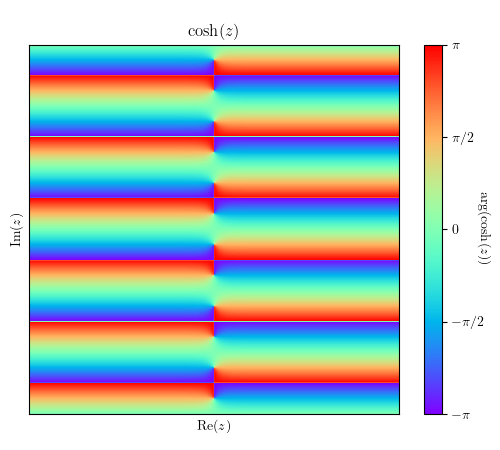
\includegraphics[scale=0.4]{cosh_phase.png}
            \caption{The phase of \(\cosh(z)\)}
        \end{subfigure}
        \begin{subfigure}{0.45\textwidth}
            \centering
            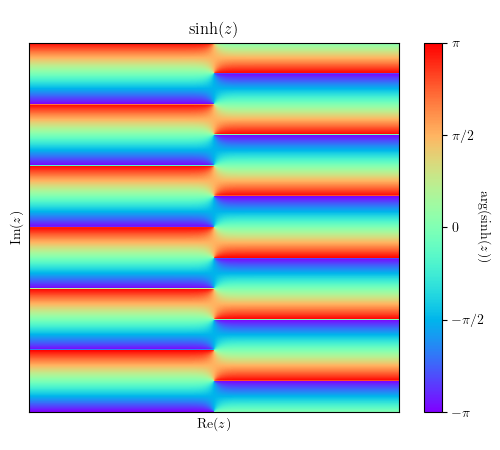
\includegraphics[scale=0.4]{sinh_phase.png}
            \caption{The phase of \(\sinh(z)\)}
        \end{subfigure}
        \begin{subfigure}{0.45\textwidth}
            \centering
            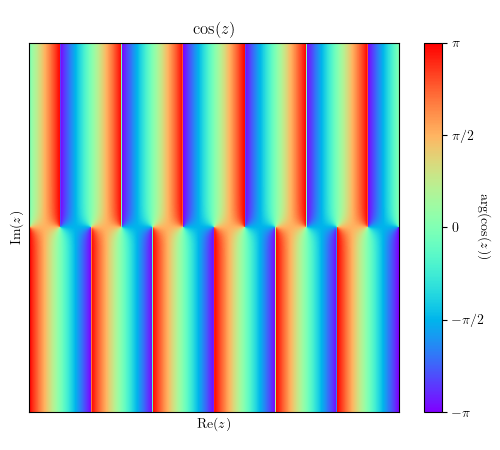
\includegraphics[scale=0.4]{cos_phase.png}
            \caption{The phase of \(\cos(z)\)}
        \end{subfigure}
        \begin{subfigure}{0.45\textwidth}
            \centering
            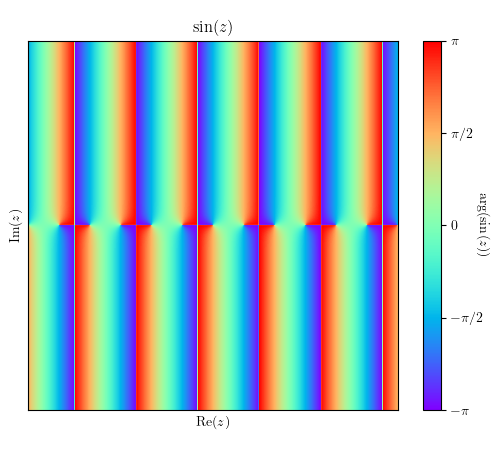
\includegraphics[scale=0.4]{sin_phase.png}
            \caption{The phase of \(\sin(z)\)}
        \end{subfigure}
        \caption{The phases of \(\cosh(z)\), \(\sinh(z)\), \(\cos(z)\), and \(\sin(z)\).}
    \end{figure}
    The following trig identities still hold for the complex versions:
    \begin{align*}
        \sin(z_1 + z_2) &= \sin(z_1)\cos(z_2) + \sin(z_2)\cos(z_1)\\
        \cos(z_1 + z_2) &= \cos(z_1)\cos(z_2) + \sin(z_1)\sin(z_2)\\
        1 &= \sin^2(z) + \cos^2(z)
    \end{align*}
    The inverse hyperbolic and trigonometric functions are given by
    \[\arcosh(z) = \log\left(z + \sqrt{z^2 - 1}\right), \qquad \arsinh(z) = \log\left(z + \sqrt{z^2 + 1}\right),\]
    \[\arccos(z) = \frac{1}{i}\log\left(z + \sqrt{1 - z^2}\right), \qquad\text{and}\qquad \arcsin(z) = \frac{1}{i}\log\left(iz + \sqrt{1 - z^2}\right).\] 
    
    \subsection{Branch Points}
    Recall that we mentioned earlier a discontinuity in \(\log(z)\) when traversing a circle about the origin.
    This is because \(z = 0\) is a branch point of \(\log z\).
    \begin{definition}{Branch point}{}
        Let \(w\colon S\subseteq\complex\to\complex\).
        We say that \(z_0\in\complex^*\) is a \define{branch point} of \(w\) if the neighbourhood, \(\discPunctured{z_0}{\varepsilon}\), contains points where \(w\) is discontinuous for arbitrarily small \(\varepsilon > 0\).
    \end{definition}
    To show that a point is a branch point it suffices to show that a circle about that point with arbitrarily small radius contains a discontinuity.
    A branch point is \emph{not} an isolated singularity as \(w\) is, by definition, continuous in the neighbourhood of an isolated singularity.
    Again notice that the value of \(w\) at \(z_0\) is unimportant in the question of whether \(z_0\) is a branch point of \(w\).
    Notice that \(z = \infty\) can be a branch point.
    We can check for this by considering the transformation \(z \to 1/t\) as \(t\to 0\).
    
    \begin{example}
        \textit{We have already seen that \(w(z) = \log z\) has a branch point at \(z = 0\).
        Does it have a branch point at \(z = \infty\)?}
        
        Make the transformation \(z \to 1/t\):
        \[\log z \to \log \frac{1}{t} = -\log t.\]
        Since this has a factor of \(\log t\) it will have a branch point at \(t = 0\) and therefore \(\log z\) has a branch point at \(z = \infty\).
    \end{example}
    \begin{example}
        \textit{Where are the branch points of \(w(z) = \sqrt{z}\)?}
        
        We can write an arbitrary real power of \(z\) as
        \[z^{\alpha} = e^{\alpha\log z} = \exp[\alpha\log\abs{z} + i\alpha(\vartheta + 2\pi n)].\]
        We see that this contains a logarithm and therefore has a branch point at \(z = 0, \infty\).
    \end{example}
    From these two examples if we have a function of square roots and logarithms we can find the branch points simply by looking for when the arguments of said logarithms and square roots are zero.
    
    \section{Branch Cuts}
    \begin{example}
        \textit{Where are the branch points of \(w(z) = \sqrt{z^2 - 1}\)?}
        
        We can write
        \[w(z) = \sqrt{z^2 - 1} = \sqrt{z - 1}\sqrt{z + 1}.\]
        First we consider when the argument of the square roots may be \(0\), we see this happens at \(z = \pm 1\).
        What about \(z = \infty\)?
        Again we make the transformation \(z \to 1/t\):
        \[\sqrt{z^2 - 1} \to \sqrt{\frac{1}{t^2} - 1} = \sqrt{\frac{1 - t^2}{t^2}} = \frac{\sqrt{1 - t^2}}{t}.\]
        Now as \(t \to 0\) this is a singularity, however that doesn't matter as the value of \(w\) is unimportant at a branch point.
        Since the argument of the square root is non-zero at \(t = 0\) this is not a branch point.
        Therefore the branch points of \(w\) are \(z = \pm 1\).
    \end{example}
    We will use this example to develop an important concept.
    A point in the plane can be expressed in polar coordinates centred at \(z = \pm 1\), see figure~\ref{fig:z in polar coords based on +/-1}.
    In these coordinates
    \[z + 1 = R^- e^{i\vartheta^-}, \qquad\text{and}\qquad z - 1 = R^{i\vartheta^+}.\]
    This allows us to express \(w(z) = \sqrt{z^2 - 1}\) as
    \[w(z) = \sqrt{z^2 - 1} = \sqrt{z + 1}\sqrt{z - 1} = \sqrt{R^+R^-}\exp\left[i\frac{1}{2}(\vartheta^+ + \vartheta^-)\right].\]
    We will use this form to investigate the discontinuities of \(w\).
    \begin{figure}[ht]
        \centering
        \tikzexternalenable
        \tikzsetnextfilename{double-polar-coordinates}
        \begin{tikzpicture}
            \tikzstyle{axis} = [thick, ->]
            \draw[axis] (-4, 0) -- (4, 0);
            \draw[axis] (0, -1) -- (0, 4);
            \coordinate (z=1) at (2, 0);
            \coordinate (z=-1) at (-2, 0);
            \coordinate (z) at (3, 3);
            \node[below] at (z=1) {\(1\)};
            \node[below] at (z=-1) {\(-1\)};
            \node[above right] at (z) {\(z\)};
            \begin{scope}
                \clip (z=1) -- (z) -- (z=-1) -- cycle;
                \draw (z=-1) circle[radius=0.5cm];
            \end{scope}
            \begin{scope}
                \clip (z=1) -- (z) -- (4, 0) -- (z=1);
                \draw (z=1) circle[radius=0.5cm];
            \end{scope}
            \draw (z=1) -- (z) node[midway, right] {\(R^+\)};
            \draw (z=-1) -- (z) node[midway, above] {\(R^-\)};
            \node at ($(z=1) + (0.68, 0.35)$) {\(\vartheta^+\)};
            \node at ($(z=-1) + (0.8, 0.2)$) {\(\vartheta^-\)};
            \draw[color=red, fill=red] (z=1) circle[radius=0.05cm]; 
            \draw[color=red, fill=red] (z=-1) circle[radius=0.05cm];
            \draw[color=green, fill=green] (z) circle[radius=0.05cm];
        \end{tikzpicture}
        \tikzexternaldisable
        \caption{A point, \(z\), can be thought of in two sets of polar coordinates centred at \(\pm 1\).}
        \label{fig:z in polar coords based on +/-1}
    \end{figure}
    What we will see is that there are discontinuities regardless of how we restrict \(\vartheta^\pm\) to have a single valued function.
    We consider three different paths across the real axis, each starting at a point \(x + i\delta\) above the axis for some \(\delta > 0\)  and ending at \(x + i\delta\) below the axis.
    If there is a discontinuity above the axis then even as \(\delta \to 0\) there will be a non-zero jump in the value of \(w\).
    
    \begin{itemize}
        \item The first choice we make is \(\vartheta^\pm \in (-\pi, \pi]\).
        \begin{itemize}
            \item The first path we consider has \(x \in (1, \infty)\).
            \subitem Above the axis in the limit \(\delta \to 0\) we have \(\vartheta^{\pm} = 0\).
            Hence
            \[\lim_{\delta\to 0} w(x + i\delta) = \sqrt{R^+R^-}\exp\left[i\frac{1}{2}(0 + 0)\right] = \sqrt{R^+R^-}.\]
            \subitem Below the axis in the limit \(\delta \to 0\) we have \(\vartheta^{\pm} \to 0\).
            Hence
            \[\lim_{\delta\to 0} w(x - i\delta) = \sqrt{R^+R^-}\exp\left[i\frac{1}{2}(0 + 0)\right] = \sqrt{R^+R^-}.\]
            Both of these are equal so there is no discontinuity in the \((1, \infty)\) interval of the real axis.
            
            \item The second path we consider has \(x \in (-1, 1)\).
            \subitem Above the axis in the limit \(\delta \to 0\) we have \(\vartheta^+ = \pi\) and \(\vartheta^- = 0\).
            Hence
            \[\lim_{\delta\to 0} w(x + i\delta) = \sqrt{R^+R^-}\exp\left[i\frac{1}{2}(\pi + 0)\right] = e^{i\pi/2}\sqrt{R^+R^-} = i\sqrt{R^+R^-}.\]
            \subitem Below the axis in the limit \(\delta \to 0\) we have \(\vartheta^+ = -\pi\) and \(\vartheta^- = 0\).
            Hence
            \[\lim_{\delta\to 0} w(x - i\delta) = \sqrt{R^+R^-}\exp\left[i\frac{1}{2}(-\pi + 0)\right] = e^{-i\pi/2}\sqrt{R^+R^-} = -i\sqrt{R^+R^-}.\]
            These are not equal so there is a discontinuity in the \((-1, 1)\) interval of the real axis.
            
            \item The third path we consider has \(x\in(-\infty, -1)\).
            \subitem Above the axis in the limit \(\delta \to 0\) we have \(\vartheta^{\pm} = \pi\).
            Hence
            \[\lim_{\delta\to 0} w(x + i\delta) = \sqrt{R^+R^-}\exp\left[i\frac{1}{2}(\pi + \pi)\right] = e^{i\pi}\sqrt{R^+R^-} = -\sqrt{R^+R^-}.\]
            \subitem Below the axis in the limit \(\delta \to 0\) we have \(\vartheta^{\pm} = -\pi\).
            Hence
            \[\lim_{\delta\to 0} w(x - i\delta) = \sqrt{R^+R^-}\exp\left[i\frac{1}{2}(-\pi + -\pi)\right] = e^{-i\pi}\sqrt{R^+R^-} = \sqrt{R^+R^-}.\]
            Both of these are equal so there is no discontinuity in the \((-\infty, 1)\) interval of the real axis.
        \end{itemize}
        We conclude that with the choice \(\vartheta^{\pm} \in (-\pi, \pi]\) there is a discontinuity only crossing the interval \((-1, 1)\) of the real axis.
        
        \item The second choice we make is \(\vartheta^+\in(-\pi, \pi]\) and \(\vartheta^-\in[0, 2\pi)\).
        \begin{itemize}
            \item The first path we consider has \(x \in (1, \infty)\).
            \subitem Above the axis in the limit \(\delta \to 0\) we have \(\vartheta^{\pm} = 0\).
            Hence
            \[\lim_{\delta\to 0} w(x + i\delta) = \sqrt{R^+R^-}\exp\left[i\frac{1}{2}(0 + 0)\right] = \sqrt{R^+R^-}.\]
            \subitem Below the axis in the limit \(\delta \to 0\) we have \(\vartheta^+ = 0\) and \(\vartheta^- = 2\pi\).
            Hence
            \[\lim_{\delta\to 0} w(x - i\delta) = \sqrt{R^+R^-}\exp\left[i\frac{1}{2}(0 + 2\pi)\right] = e^{i\pi}\sqrt{R^+R^-} = -\sqrt{R^+R^-}.\]
            These are not equal so there is a discontinuity in the \((1, \infty)\) interval of the real axis.
            
            \item The second path we consider has \(x\in(-1, 1)\).
            \subitem Above the axis in the limit \(\delta \to 0\) we have \(\vartheta^+ = -\pi\) and \(\vartheta^- = 2\pi\).
            Hence
            \[\lim_{\delta\to 0} w(x + i\delta) = \sqrt{R^+R^-}\exp\left[i\frac{1}{2}(2\pi - \pi)\right] = e^{i\pi/2}\sqrt{R^+R^-} = i\sqrt{R^+R^-}.\]
            \subitem Below the axis in the limit \(\delta \to 0\) we have \(\vartheta^+ = -\pi\) and \(\vartheta^- = 2\pi\).
            Hence
            \[\lim_{\delta\to 0} w(x - i\delta) = \sqrt{R^+R^-}\exp\left[i\frac{1}{2}(-\pi + 2\pi)\right] = e^{i\pi/2}\sqrt{R^+R^-} = i\sqrt{R^+R^-}.\]
            Both of these are equal so there is no discontinuity in the \((-1, 1)\) interval of the real axis.
            
            \item The third path we consider has \(x\in(-\infty, -1)\).
            \subitem Above the axis in the limit \(\delta \to 0\) we have \(\vartheta^{\pm} = \pi\).
            Hence
            \[\lim_{\delta\to 0} w(x + i\delta) = \sqrt{R^+R^-}\exp\left[i\frac{1}{2}(\pi + \pi)\right] = e^{i\pi}\sqrt{R^+R^-} = \sqrt{R^+R^-}.\]
            \subitem Below the axis in the limit \(\delta \to 0\) we have \(\vartheta^+ = -\pi\) and \(\vartheta^- = \pi\).
            Hence
            \[\lim_{\delta\to 0} w(x - i\delta) = \sqrt{R^+R^-}\exp\left[i\frac{1}{2}(-\pi + \pi)\right] = \sqrt{R^+R^-}.\]
            These are not equal so there is a discontinuity in the \((-\infty, 1)\) interval of the real axis.
        \end{itemize}
        We conclude that with the choice \(\vartheta^+\in(-\pi, \pi]\) and \(\vartheta^-\in[0, 2\pi)\) there is a discontinuity crossing the real axis in either \((-\infty, -1)\) or \((1, \infty)\).
    \end{itemize}
    This demonstrates the importance of choosing the argument.
    In general it is possible to move discontinuities by changing the argument but we cannot get rid of them.
    There is no `right answer', it is best to make a choice and write it down and be careful to stick with it.
    
    \begin{definition}{Branch cut}{}
        A \define{branch cut} is an arbitrary path that joins two branch points and as a result of which the function in question becomes single valued.
    \end{definition}
    Figure~\ref{fig:sqrt z riemann surface} shows a Riemann surface, which is a way of plotting complex functions.
    This one shows \(\sqrt{z}\) which we can see is multi valued.
    We can think of branch points as the points where multiple sheets coincide.
    Figure~\ref{fig:sqrt z riemann surface with branch cut} shows the same Riemann surface after a branch cut along the negative real axis, which joins \(0\) and \(\infty\), the two branch points of \(\sqrt{z}\).
    The function is now single valued and the discontinuity at the branch cut is fairly obvious.
    \begin{figure}[ht]
        \centering
        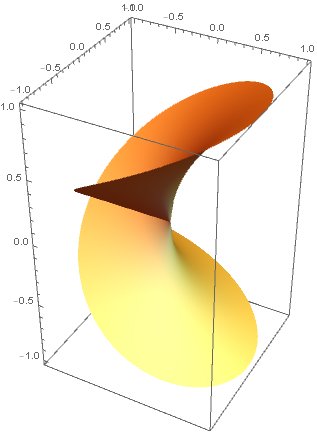
\includegraphics[scale=0.6]{sqrt_z_riemann_surface.png}
        \caption{The Riemann surface of \(\sqrt{z}\) showing the real and imaginary parts in the bottom plane and \(\Re(\sqrt{z})\) in the vertical axis.}
        \label{fig:sqrt z riemann surface}
    \end{figure}
    \begin{figure}[ht]
        \centering
        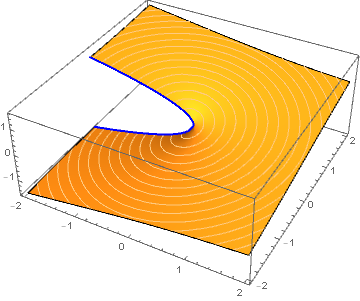
\includegraphics[scale=0.6]{sqrt_z_riemann_surface_with_branch_cut.png}
        \caption{The Riemann surface of \(\sqrt{z}\) with a branch cut along the negative real axis in order to make the function single valued. The branch cut is shown in blue.}
        \label{fig:sqrt z riemann surface with branch cut}
    \end{figure}
    
    \begin{figure}[ht]
        \centering
        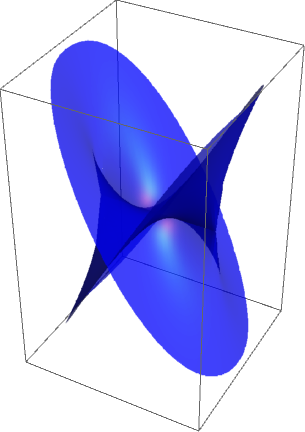
\includegraphics[scale=0.6]{sqrt_z_squared_minus_1_riemann_surface.png}
        \caption{The Riemann surface of \(\sqrt{z^2 - 1}\) with two branch points at \(z = \pm 1\).}
    \end{figure}
    \begin{figure}[ht]
        \centering
        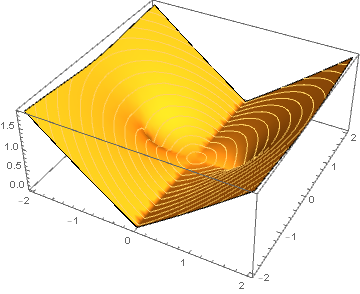
\includegraphics[scale=0.6]{sqrt_z_squared_minus_1_riemann_surface_with_branch_cuts}
        \caption{The Riemann surface of \(\sqrt{z^2 - 1}\) with a branch point from \(z = \infty\) to \(z = \pm 1\). Essentially this cuts the bottom half off to make the function single valued.}
    \end{figure}

    \part{Integrals}
    \section{Complex Integration}
    \subsection{Integrating Functions From \texorpdfstring{\(\reals\)}{R} to \texorpdfstring{\(\complex\)}{C}}
    Before we define integration in the complex plane we consider a simpler case.
    Consider a function, \(w\colon\reals\to\complex\).
    We can write this function as
    \[w(t) = u(t) + iv(t)\]
    where \(u, v\colon\reals\to\reals\).
    If \(u\) and \(v\) are both piecewise continuous (that is contain a countable number of discontinuities) then we can integrate \(w\) the same way we would integrate a real integral.
    For example integrating over \((a, b)\) we have
    \[\int_a^b w(t) \dd{t} = \int_a^b u(t)\dd{t} + i\int_a^b v(t) \dd{t} = [U(t) + iV(t)]_a^b\]
    where \(U\) and \(V\) are the antiderivatives of \(u\) and \(v\).
    This simplified case of integrating only along \(\reals\) actually turns out to be very close to the more common case of a function defined on a particular path in the complex plane.
    We simply need to parametrise the path with a real parameter and then complex integrals become remarkably similar to their real counterpart.
    For example the integral as defined above is linear, that is for \(\alpha, \beta\in\complex\) and piecewise continuous functions \(f, g\colon\reals\to\complex\)
    \[\int_a^b [\alpha f(t) + \beta g(t)] \dd{t} = \alpha \int_a^b f(t) \dd{t} + \beta \int_a^b g(t) \dd{t}.\]
    
    \subsection{Arcs and Contours}
    The main difference between integrating a function defined on \(\reals\) and a function defined on \(\complex\) is that in the second case there are multiple paths we can take to get from \(a\) to \(b\).
    We have to define the path we are integrating along and in general it makes a difference which path we choose.
    This should be familiar from line integrals from multivariable calculus.
    In the complex plane we define a contour to integrate along.
    There are a few restraints on what paths we can choose as a contour.
    \begin{definition}{Smooth arc}{}
        The set of points
        \[\{\gamma(t) = x(t) + iy(t) \st x, y\colon\reals\to\reals\wedge t\in(a, b)\subseteq\reals\}\]
        is a \define{smooth arc} with end points \(\{a, b\}\) if both \(x(t)\) and \(y(t)\) are continuous and differentiable and \(\gamma'(t) = x'(t) + iy'(t) \ne 0\) for all \(t\in(a, b)\).
    \end{definition}
    \begin{notation*}{}
        We denote by \(C^k(X)\) the set of all functions defined on \(X\) with at least \(k\) continuous derivatives (on some domain of interest).
        Often we write \(C^k\) when the domain is obvious.
        For example \(C^0\) is the set of continuous functions which may or may not be differentiable and \(C^1\) is the set of differentiable functions with continuous derivatives. 
        Note that since we define \(f\in C^k\) to have at least \(k\) continuous derivatives we also know that \(f\in C^{k'}\) for all \(k'\le k\), for example the function defined by \(f(z) = e^z\) is in \(C^{\infty}\) but it is also in \(C^k\) fo all \(k\in\naturals\).
    \end{notation*}
    \begin{definition}{Contour}{}
        A \define{contour}, \(\gamma\), is a continuous chain of a finite number of smooth arcs.
        We say that \(\gamma\) is piecewise smooth.
    \end{definition}
    The condition that the number of arcs is finite is important.
    \begin{example}\label{exa:contours}
        Consider the path defined by
        \[\gamma(t) = z_0 + te^{i\vartheta}, \qquad t\in(0, 1)\]
        for some constant \(\vartheta\).
        To see what this arc looks like consider \(\gamma(0) = z_0\) and \(\gamma(1) = z_0 + e^{i\vartheta}\).
        This arc corresponds to a straight line between these two points as can be seen in figure~\ref{fig:contour example 1}.
        Notice that \(\gamma'(t) = e^{i\vartheta}\) is non-zero for all finite \(\vartheta\) so \(\gamma\) is a smooth arc.
        
        Consider the path defined by
        \[\gamma(t) = z_0 + Re^{it}, \qquad t\in(0, \pi/2)\]
        for some constant \(R\).
        To see what this arc looks like consider \(\gamma(0) = z_0 + R\) and \(\gamma(1) = z_0 + iR\).
        This arc corresponds to an arc (in the part of a circle sense) centred on \(z_0\) with radius \(R\) starting at 0 and going round to \(\pi/2\) as can be seen in figure~\ref{fig:contour example 2}.
        Notice that \(\gamma'(t) = iRe^it\) is non-zero for all finite \(t\) so \(\gamma\) is a smooth arc.
        
        Consider the path defined by
        \[\gamma(t) = t + ie^{-it}, \qquad t\in(0, 3\pi).\]
        Notice that
        \[\Re(z) = t + \cos t, \qquad\text{and}\qquad \Im(z) = 1 - \sin t\]
        so
        \[z'(t) = 1 - \sin t - i\cos t.\]
        This is zero for \(t = \pi/2 + 2n\pi\), \(n\in\integers\).
        Therefore this is \emph{not} a smooth arc.
        However as we see in figure~\ref{fig:contour example 3} we can decompose it into three smooth arcs which makes it a valid contour.
        \tikzexternalenable
        \begin{figure}[ht]
            \centering
            \begin{subfigure}{0.4\textwidth}
                \centering
                \tikzsetnextfilename{contour_example_1}
                \begin{tikzpicture}
                    \tikzstyle{contour} = [very thick]
                    \draw[contour] (0, 0) -- (2, 2);
                    \draw[fill=black] (0, 0) circle[radius=0.05cm] node[below left] {\(z_0\)};
                    \draw[fill=black] (2, 2) circle[radius=0.05cm] node[above right] {\(z_0 + e^{i\vartheta}\)};
                    \begin{scope}
                        \clip (0, 0) -- (2, 2) -- (2, 0) -- cycle;
                        \draw (0, 0) circle[radius=0.5cm];
                    \end{scope}
                    \node at (0.6, 0.2) {\(\vartheta\)};
                    \draw[dashed] (0, 0) -- (1, 0);
                \end{tikzpicture}
                \caption{The contour defined by \(\gamma(t) = z_0 + te^{i\vartheta}\) for \(t\in(0, 1)\).}
                \label{fig:contour example 1}
            \end{subfigure}
            \begin{subfigure}{0.4\textwidth}
                \centering
                \tikzsetnextfilename{contour_example_2}
                \begin{tikzpicture}
                    \tikzstyle{contour} = [very thick]
                    \draw[fill=black] (0, 0) circle[radius=0.05cm] node[below left] {\(z_0\)};
                    \draw[fill=black] (2, 0) circle[radius=0.05cm] node[below] {\(z_0 + R\)};
                    \draw[fill=black] (0, 2) circle[radius=0.05cm] node[above] {\(z_0 + iR\)};
                    \begin{scope}
                        \clip (0, 0) -- (3, 0) -- (3, 3) -- (0, 3) -- cycle;
                        \draw[contour] (0, 0) circle[radius=2cm];
                    \end{scope}
                    \draw[dashed] (0, 2) -- (0, 0) -- (2, 0);
                    \draw (0.5, 0) -- (0.5, 0.5) -- (0, 0.5);
                \end{tikzpicture}
                \caption{The contour defined by \(\gamma(t) = z_0 + Re^{it}\) for \(t\in(0, \pi/2)\).}
                \label{fig:contour example 2}
            \end{subfigure}
            \begin{subfigure}{0.9\textwidth}
                \centering
                \tikzsetnextfilename{contour_example_3}
                \begin{tikzpicture}
                    \tikzstyle{contour} = [very thick]
                    \begin{axis}[xmin=0,xmax=10, samples=50, axis equal image, hide axis]
                        \addplot[contour, red, domain=0:1.571] ({x + cos(deg(x))}, {1 - sin(deg(x))});
                        \addplot[contour, blue, domain=1.571:7.854] ({x + cos(deg(x))}, {1 - sin(deg(x))});
                        \addplot[contour, green, domain=7.854:9.42] ({x + cos(deg(x))}, {1 - sin(deg(x))});
                    \end{axis}
                \end{tikzpicture}
                \caption{The contour defined by \(\gamma(t) = t + i + e^{-it}\) for \(t\in(0, 3\pi)\). Different colours are used to plot the three smooth arcs that make up the contour. The smooth arcs start and end at the points where \(\gamma'(t) = 0\) which is \(\pi/2 + 2n\pi\) for \(n\in\integers\).}
                \label{fig:contour example 3}
            \end{subfigure}
            \caption{Various examples of contours.}
        \end{figure}
        \tikzexternaldisable
    \end{example}
    \subsection{The Integral}
    \begin{definition}{Integral}{}
        Let \(\gamma\) be a contour.
        We split \(\gamma\) into \(n\) sections and define \(\{z_{\alpha}\}\) as the set of \(n + 1\) end points of each section.
        Let \(w\colon\complex\to\complex\) be a piecewise continuous complex function.
        Define the sum
        \[S_n = \sum_{\alpha = 1}^{n} w(z_\alpha)(z_{\alpha} - z_{\alpha - 1}).\]
        Now let \(n\to\infty\) and let the length of each segment \(\abs{z_\alpha - z_{\alpha - 1}} \to 0\).
        If this limit exists we say that \(w\) is \define{integrable} on \(\gamma\).
        In this case the limit is called the \define{integral} of \(w\) on \(\gamma\), or in the normal notation
        \[ \lim_{n\to\infty} S_n = \int_\gamma w(z) \dd{z}.\]
    \end{definition}
    \begin{lemma}{Linearity of the integral}{}
        Let \(\gamma\) be a contour, let \(f\) and \(g\) be piecewise continuous functions on \(\gamma\), and let \(\alpha, \beta\in\complex\) be constants.
        Then
        \[\int_\gamma (\alpha f(z) + \beta g(z)) \dd{z} = \alpha \int_\gamma f(z) \dd{z} + \beta \int_\gamma g(z) \dd{z}.\]
    \end{lemma}
    \begin{proof}
        Split the contour \(\gamma\), as in the definition of the integral, into \(n\) sections with end points \(z_{i}\) and length \(\abs{z_{i} - z_{i - 1}}\) such that the of each interval vanishes as \(n \to \infty\).
        Then
        \begin{align*}
            \int_\gamma (\alpha f(z) + \beta g(z)) \dd{z} &= \lim_{n\to\infty} \left[(\alpha f(z_{i}) \beta g(z_i))(z_i - z_{i-1})\right]\\
            &= \lim_{n\to\infty} \left[\alpha f(z_{i})(z_i - z_{i-1}) \beta g(z_i)(z_i - z_{i-1})\right]\\
            &= \alpha\lim_{n\to\infty} f(z_{i})(z_i - z_{i-1}) \beta\lim_{n\to\infty} g(z_i)(z_i - z_{i-1})\\
            &= \alpha \int_\gamma f(z) \dd{z} + \beta \int_\gamma g(z) \dd{z}.
        \end{align*}
        Here we have used the fact that
        \[\lim_{n\to\infty} [aA_n + bB_n] = a\lim_{n\to\infty}A_n + b\lim_{n\to\infty}B_n\]
        for some convergent complex sequences \((A_n)\) and \((B_n)\) and complex constants \(a\) and \(b\).
    \end{proof}
    \begin{definition}{Closed contour}{}
        Let \(\gamma\) be a contour with endpoints \(a\) and \(b\).
        If \(a = b\) we say that the contour is \define{closed}.
    \end{definition}
    Note that this sort of closed is not the same as the topological sort of closed (i.e. that the set contains its boundary).
    \begin{notation*}{}
        If \(\gamma\) is a closed contour and \(w\) is integrable on \(\gamma\) then we denote the integral by
        \[\oint_{\gamma} w(z) \dd{z}.\]
        As a matter of convention when integrating along a closed contour we go anticlockwise.
    \end{notation*}
    
    \subsection{Evaluating Integrals}
    Now that we have defined an integral we can start actually integrating things.
    Let \(\{\gamma_k\}\) be smooth arcs which together form a contour, \(\gamma\).
    Let \(\gamma_k\) be parametrised by some real variable \(t \in (a, b)\).
    Under this parametrisation the points on \(\gamma_k\) can be written as \(z = z[\gamma_k(t)] = x(t) + iy(t)\) where \(x, y\colon\reals\to\reals\).
    Differentiating we have
    \[\dv{z}{t} = x'(t) + iy'(t) = \gamma_k'(t) \implies \dd{z} = [x'(t) + iy(t)]\dd{t} = \gamma_k'(t)\dd{t}.\]
    Now let \(w\colon\complex\to\complex\) be integrable on \(\gamma\) and let \(w(\gamma(t)) = u(t) + iv(t)\) where \(u, v\colon\reals\to\reals\).
    Then the substitution \(z\to\gamma_k\) gives us
    \begin{align*}
        \int_{\gamma_k} w(z)\dd{z} &= \int_a^b w[\gamma_k(t)] \gamma_k'(t) \dd{t}\\
        &= \int_a^b [u(t) + iv(t)][x'(t) + iy'(t)] \dd{t}\\
        &= \int_a^b [u(t)x'(t) - v(t)y'(t)]\dd{t} + i\int_a^b [v(t)x'(t) + u(t)y'(t)]\dd{t}.
    \end{align*}
    These integrals can then be easily evaluated using techniques from real integral calculus.
    
    \begin{lemma}{Integral properties}{}
        Let \(\gamma\) be a piecewise smooth contour and let \(f\) be a continuous function on \(\gamma\).
        Then the following hold.
        \begin{enumerate}
            \item Inverting the contour inverts the integral:
            \[\int_{-\gamma} f(z) \dd{z} = -\int_{\gamma} f(z) \dd{z}.\]
            
            \item If \(\gamma\) can be decomposed into two smooth contours \(\gamma_1\) and \(\gamma_2\) then
            \[\int_\gamma f(z) \dd{z} = \int_{\gamma_1} f(z) \dd{z} + \int_{\gamma_2} f(z) \dd{z}.\]
            
            \item Two different parametrisations of \(\gamma\) will yield the same result.
            That is if \(\gamma_1\) and \(\gamma_2\) are smooth arcs with endpoints \(\{a, b\}\) and \(\{a', b'\}\) respectively and \(g\colon(a, b) \to (a', b')\) such that \(g(\gamma_1) = \gamma_2\) then
            \[\int_{\gamma_1} f(z) \dd{z} = \int_{\gamma_2} f(z) \dd{z}.\]
        \end{enumerate}
    \end{lemma}
    \begin{proof}
        ~  % Forces a space which makes enumerate start on a new line.
        \begin{enumerate}
            \item Consider the definition of the integral over \(\gamma\)
            \begin{align*}
                -\int_{\gamma}f(z)\dd{z} &= -\lim_{n\to\infty} \sum_{\alpha=1}^{n} f(z_{\alpha})(z_{\alpha}-z_{\alpha-1})\\
                &= \lim_{n\to\infty} \sum_{\alpha=1}^{n} f(z_{\alpha})(z_{\alpha-1}-z_{\alpha})\\
                &= \int_{-\gamma} f(z) \dd{z}.
            \end{align*}
            This proves the first statement.
            
            An alternative proof of this statement can be given by parametrising the contour.
            Consider a parametrisation of \(\gamma\) by some real variable \(t\in(0, 1)\) and notice that \(-\gamma\) is then parametrised by the same parametrisation with \(1 - t'\) where \(t'\in(0, 1)\).
            The end points are inverted but it is the same set of points.
            Hence
            \begin{align*}
                \int_{-\gamma} f(z) \dd{z} &= -\int_{t'=0}^{t'=1} f[\gamma(1 - t')]\gamma'(1 - t')\dd{t'}\\
                &= \int_{t'=1}^{t'=0} f[\gamma(1 - t')]\gamma'(1 - t')\dd{t'}
                \shortintertext{nows substituting \(1 - t' = t\)}
                &= -\int_{t=0}^{t=1} f[\gamma(t)]\gamma'(t)\dd{t}\\
                &= -\int_{\gamma} f(z)\dd{z}.
            \end{align*}
            This proves the property also.
            
            \item Let \(\gamma\) be parametrised by a real variable \(t\in[a, b]\).
            Let \(c\) be such that \(\gamma(t)\) corresponds to a point on \(\gamma_1\) if \(t\in(a, c)\) and a point on \(\gamma_2\) if \(t\in(c, b)\).
            The integrals of the real and imaginary parts of \(f\) behave like real integrals and we know for a real integral of some integrable function \(h\) on \((a, b)\) that
            \[\int_a^b h(t)\dd{t} = \int_a^c h(t) \dd{t} + \int_c^b h(t) \dd{t}\]
            where \(a \le c \le b\).
            Applying this to the real and complex parts of the integral of \(f\) we have
            \[\int_a^b f[\gamma(t)]\gamma'(t) = \int_a^c f[\gamma_1(t)]\gamma_1'(t)\dd{t} + \int_c^b f[\gamma_1(t)]\gamma_2'(t)\dd{t}.\]
            Hence
            \[\int_\gamma f(z) \dd{z} = \int_{\gamma_1} f(z) \dd{z} + \int_{\gamma_2} f(z)\dd{z}.\]
            This proves the second property.
            
            \item For the final property we have
            \begin{align*}
                \int_{\gamma_2} f(z) \dd{z} &= \int_{a'}^{b'} f[\gamma_2(t)]\gamma_2'(t)\dd{t}\\
                &= \int_{a'}^{b'} f\{g[\gamma_1(t)]\}\dv{g[\gamma_1(t)]}{t}\dd{t}\\
                &= \int_{a'}^{b'} f\{g[\gamma_1(t)]\}\dd{g[\gamma_1(t)]}
                \shortintertext{making the substitution \(g[\gamma_2(t)] \to \gamma_1(t)\) we have \(\dd{t'} = \dd{g[\gamma_2]}\) so we get}
                &= \int_a^b f[\gamma_1(t')]\gamma_1'(t)\dd{t'}\\
                &= \int_{\gamma_1} f(z) \dd{z}.
            \end{align*}
            This proves the third property.
        \end{enumerate}
    \end{proof}
    
    \subsubsection{Evaluating Integrals Examples}
    With these properties we are finally ready for some examples.
    \begin{example}\label{exa:integral 1}
        \textit{
            Let \(f(z) = z^2\).
            Find the integral
        }
            \[\int_{\gamma} z^2 \dd{z}\]
        \textit{
            where \(\gamma\) is one of the following contours:
        }
        \begin{enumerate}[label=\textit{\arabic*.}]
            \item \textit{a straight line segment from \(0\) to \(1 + i\),}
            \item \textit{two straight line segments from \(0\) to 1 and from 1 to \(1 + i\).}
        \end{enumerate}

        \begin{enumerate}
            \item We can parametrise the first contour as \(\gamma(t) = t(1 + i)\) with \(t\in(0, 1)\).
            Then \(\gamma'(t) = 1 + i\), which is non-zero as required.
            The integral is then
            \[\int_\gamma z^2 \dd{z} = \int_0^1 [t(1 + i)]^2(1 + i) \dd{t} = (1 + i)^3\int_0^1 t^2\dd{t} = (1 + i)^3\left[\frac{1}{3}t^3\right]_0^1 = (1 + i)^3\frac{1}{3} = \frac{-2 + 2i}{3}.\]
            
            \item The second contour can be parametrised in two parts by \(\gamma_1(t) = t\) for \(t\in(0, 1)\) and \(\gamma_2(t) = 1 + it\) for \(t\in(0, 1)\).
            The derivatives of the contours are \(\gamma_1'(t) = 1\) and \(\gamma_2'(t) = i\) which are both non-zero as required.
            Integrating over these contours we have
            \[\int_{\gamma_1} z^2\dd{z} = \int_0^1 t^2 \dd{t} = \frac{1}{3}\]
            and
            \[\int_{\gamma_2} z^2 \dd{z} = \int_0^1 (1 + it)^2i\dd{t} = i\int_0^t (1 - t^2 + 2it)\dd{t} = -1 + \frac{2i}{3}.\]
            Thus the integral along the whole contour is
            \[\int_{\gamma_1}z^2\dd{z} + \int_{\gamma_2}z^2\dd{z} = \frac{-2 + 2i}{3}.\]
        \end{enumerate}
        Notice that both contours gave the same result.
        This is not the case in general as we will see in the next example.
    \end{example}
    \begin{example}\label{exa:integral 2}
        \textit{
            Let \(f(z) = 1/z\).
            Find the integral
        }
            \[\int_{\gamma} \frac{1}{z} \dd{z}\]
        \textit{
            where \(\gamma\) is one of the following contours
        }
        \begin{enumerate}[label=\textit{\arabic*.}]
            \item \textit{\(\gamma_1\), the upper semicircle from \(-1\) to 1,}
            \item \textit{\(\gamma_2\), the lower semicircle from \(-1\) to 1.}
        \end{enumerate}
        \begin{enumerate}
            \item \(\gamma_1\) can be parametrised as \(\gamma_1(t) = e^{it}\) where \(t\in(0, \pi)\).
            Note that for the direction to be from \(-1\) to 1 we need to start at \(t = \pi\).
            The derivative of this contour parametrisation is \(\gamma'(t) = ie^{it}\) which is non-zero on \((0, \pi)\) as required.
            The integral is then
            \[\int_{\gamma_1} \frac{1}{z}\dd{z} = \int_{\pi}^{0} \frac{1}{e^{it}}ie^{it}\dd{t} = i\in_\pi^0 \dd{t} = -i\pi.\]
            
            \item \(\gamma_2\) can be parametrised as \(\gamma_2(t) = e^{it}\) where \(t\in(-\pi, 0)\).
            The derivative of this contour parametrisation is \(\gamma'(t) = ie^{it}\) which is non-zero on \((-\pi, 0)\) as required.
            The integral is then
            \[\int_{\gamma_2} \frac{1}{z}\dd{z} = \int_{-\pi}^{0} \frac{1}{e^{it}}ie^{it}\dd{t} = i\in_{-\pi}^0 \dd{t} = i\pi.\]
        \end{enumerate}
        We see that the value of the integral depends on the contour chosen.
    \end{example}
    \begin{example}\label{exa:integral 3}
        \textit{
            Let \(f(z) = \abs{z}^2\).
            Find the integral
        }
            \[\int_\gamma f(z)\dd{z}\]
        \textit{
            where \(\gamma\) is one of the following contours
        }
        \begin{enumerate}[label=\textit{\arabic*.}]
            \item \textit{\(\gamma_1\), a straight segment from \(-1\) to \(i\),}
            \item \textit{\(\gamma_2\), a \(\pi/2\) circular arc of radius 1 from \(-1\) to \(i\).}
        \end{enumerate}
        \begin{enumerate}
            \item \(\gamma_1\) can be parametrised as \(\gamma_1(t) = -1 + (1 + i)t\) with \(t\in(0, 1)\).
            The derivative of this contour parametrisation is \(\gamma_1'(t) = 1 + i\) which is non-zero as required.
            The integral is then
            \[\int_{\gamma_1} \abs{z}^2 = \int_0^1 \abs{t - 1 + it}(1 + i)\dd{t} = (1 + i)\int_0^1 [(t - 1)^2 + t^2] \dd{t} = \frac{2}{3}(1 + i).\]
            
            \item \(\gamma_2\) can be parametrised as \(\gamma_2(t) = e^{it}\) where \(t\in(\pi/2, \pi)\).
            Note that for the direction to be from \(-1\) to \(i\) we need to start at \(t = \pi\).
            The derivative of this contour parametrisation is \(\gamma'(t) = ie^{it}\) which is non-zero on \((\pi/2, \pi)\) as required.
            The integral is then
            \[\int_{\gamma_2} \abs{z}^2\dd{z} = \int_{\pi}^{\pi/2} \abs{e^{it}}^2 ie^{it} \dd{t} = \int_{\pi}^{\pi/2} ie^{it} \dd{t} = i + 1.\]
        \end{enumerate}
        Again we see that the result depends on the contour.
    \end{example}
    \begin{figure}[ht]
        \centering
        \tikzexternalenable
        \begin{subfigure}{0.4\textwidth}
            \centering
            \tikzsetnextfilename{integral-example-1}
            \begin{tikzpicture}
                \tikzstyle{contour} = [ultra thick, color={#1}]
                \tikzstyle{axis} = [very thick, ->]
                \tikzstyle{point} = [fill=black]
                \draw[axis] (0, -1.5) -- (0, 1.5) node[above] {\(\Im\)};
                \draw[axis] (-1.5, 0) -- (1.5, 0) node[right] {\(\Re\)};
                \draw[contour=red] (0, 0) -- (1, 1);
                \draw[contour=red, ->] (0, 0) -- (0.5, 0.5);
                \draw[contour=blue] (0, 0) -- (1, 0);
                \draw[contour=blue, ->] (0, 0) -- (0.5, 0);
                \draw[contour=blue] (1, 0) -- (1, 1);
                \draw[contour=blue, ->] (1, 0) -- (1, 0.5);
                \draw[point] (0, 0) circle[radius=0.05cm];
                \draw[point] (1, 1) circle[radius=0.05cm];
            \end{tikzpicture}
            \caption{The contours in example~\ref{exa:integral 1}}
        \end{subfigure}
        \begin{subfigure}{0.4\textwidth}
            \centering
            \tikzsetnextfilename{integral-example-2}
            \begin{tikzpicture}
                \tikzstyle{contour} = [ultra thick, color={#1}]
                \tikzstyle{axis} = [very thick, ->]
                \tikzstyle{point} = [fill=black]
                \draw[axis] (0, -1.5) -- (0, 1.5) node[above] {\(\Im\)};
                \draw[axis] (-1.5, 0) -- (1.5, 0) node[right] {\(\Re\)};
                \draw[contour=red] (-1, 0) arc(180:0:1);
                \draw[contour=red, ->] (-1, 0) arc(180:135:1);
                \draw[contour=red, ->] (-1, 0) arc(180:45:1);
                \draw[contour=blue] (-1, 0) arc(-180:0:1);
                \draw[contour=blue, ->] (-1, 0) arc(-180:-135:1);
                \draw[contour=blue, ->] (-1, 0) arc(-180:-45:1);
                \draw[point] (-1, 0) circle[radius=0.05cm];
                \draw[point] (1, 0) circle[radius=0.05cm];
            \end{tikzpicture}
            \caption{The contours in example~\ref{exa:integral 2}}
        \end{subfigure}
        \begin{subfigure}{0.4\textwidth}
            \centering
            \tikzsetnextfilename{integral-example-3}
            \begin{tikzpicture}
                \tikzstyle{contour} = [ultra thick, color={#1}]
                \tikzstyle{axis} = [very thick, ->]
                \tikzstyle{point} = [fill=black]
                \draw[axis] (0, -1.5) -- (0, 1.5) node[above] {\(\Im\)};
                \draw[axis] (-1.5, 0) -- (1.5, 0) node[right] {\(\Re\)};
                \draw[contour=red] (-1, 0) -- (0, 1);
                \draw[contour=red, ->]  (-1, 0) -- (-0.5, 0.5);
                \draw[contour=blue] (-1, 0) arc(180:90:1);
                \draw[contour=blue, ->] (-1, 0) arc(180:135:1);
            \end{tikzpicture}
            \caption{The contours in example~\ref{exa:integral 2}}
        \end{subfigure}
    \tikzexternaldisable
    \end{figure}
    
    \section{Cauchy's Integral Theorem}
    \subsection{Bounding Integrals}
    \begin{lemma}{Integral bound}{integral bound}
        Let \(\gamma\) be a contour and let \(f\) be a piecewise continuous function on \(\gamma\).
        Then
        \[\abs{\int_{\gamma} f(z) \dd{z}} \le \int_{\gamma} \abs{f(z) \dd{z}} = \int_{\gamma} \abs{f(z)}\abs{\dd{z}}.\]
    \end{lemma}
    \begin{proof}
        Let
        \[I = \int_\gamma f(z) \dd{z}.\]
        Since this is a complex integral in general \(I\in\complex\).
        Therefore we can write \(I\) as \(I = Re^{i\vartheta}\).
        This lemma is interested in providing a bound on \(R = \abs{I}\).
        Note that \(e^{-i\vartheta}I = e^{-i\vartheta}Re^{i\vartheta} = R\) and that \(\abs{e^{i\vartheta}} = 1\).
        Then
        \begin{align*}
            \abs{\int_{\gamma} f(z) \dd{z}} &= e^{i\vartheta} \int_\gamma f(z) \dd{z}\\
            &= \int_{\gamma} e^{-i\vartheta} f(z) \dd{z}.
        \end{align*}
        The integral in the last step is real since it is equal to the absolute value of another integral.
        This means we can take the real part without changing anything so
        \begin{align*}
            \abs{\int_{\gamma} f(z) \dd{z}} &= \Re\left[\int_\gamma e^{-i\vartheta} f(z)\dd{z}\right]\\
            &= \int_{\gamma} \Re[e^{-i\vartheta} f(z)\dd{z}]
        \end{align*}
        Now we use \(\Re(z) \le \abs{z}\) from the first point of theorem~\ref{lem:modulus inequalities} and we get
        \begin{align*}
            \abs{\int_{\gamma} f(z) \dd{z}} &\le \int_\gamma \abs{e^{-i\vartheta}f(z)\dd{z}}\\
            &= \int_{\gamma} \abs{f(z) \dd{z}}\\
            &= \int_{\gamma} \abs{f(z)} \abs{\dd{z}}.
        \end{align*}
    \end{proof}
    Note that we have to take the absolute value of the measure, \(\dd{z}\), for this inequality to hold.
    This will be important in the next lemma.
    Consider
    \[\int_{\gamma} \abs{\dd{z}}\]
    for some contour \(\gamma\).
    Appealing to the definition of the integral this is simply
    \[\int_{\gamma} \abs{\dd{z}} = \lim_{N\to\infty} \sum_{i=1}^{N}\abs{z_{i} - z_{i-1}}.\]
    That is the sum of the length of all of the segments of the contour, which when summed just gives the length of the contour, \(L\).
    
    \begin{lemma}{ML lemma}{ML lemma}
        Let \(\gamma\) be a contour on \(\complex\) with length \(L\).
        Let \(f\) be a function that is piecewise continuous on \(\gamma\).
        Let \(M\) be a real constant that bounds \(\abs{f(z)}\) on \(\gamma\).
        That is for all \(z\in\gamma\) \(M \ge \abs{f(z)}\).
        Then
        \[\abs{\int_\gamma f(z)\dd{z}} \le ML.\]
    \end{lemma}
    \begin{proof}
        By lemma~\ref{lem:integral bound} we know that
        \[\abs{\int_\gamma f(z)\dd{z}} \le \int_{\gamma} \abs{f(z)} \abs{\dd{z}}.\]
        Clearly if we replace \(\abs{f(z)}\) with \(M\) the value of the integral can only increase.
        Therefore
        \[\abs{\int_\gamma f(z)\dd{z}} \le \int_{\gamma} M\abs{\dd{z}} = M\int_{\gamma} \abs{\dd{z}} = ML.\]
    \end{proof}
    
    \begin{example}
        \textit{Let \(\alpha\in\reals\). Show, using integral bounds, that \(\abs{\exp(2\pi\alpha i) - 1} \le 2\pi\abs{\alpha}\).}
        
        If \(\alpha = 0\) then equality holds.
        Therefore assume \(\alpha \ne 0\).
        We consider
        \[\int_{\gamma}e^{i\alpha z}\dd{z}\]
        where \(\gamma\) is a straight line from \(0\) to \(2\pi\).
        Applying a bound to the integral we have
        \[\abs{\int_{\gamma} e^{i\alpha z}\dd{z}} \le \int_{\gamma} \abs{e^{-i\alpha z}\dd{z}} = \int_0^{2\pi} \abs{e^{i\alpha t}}\dd{t} = \int_0^{2\pi}\dd{t} = 2\pi.\]
        Evaluating the integral instead gives
        \[\abs{\int_{\gamma} e^{i\alpha z}\dd{z}} = \abs{\int_0^{2\pi} e^{i\alpha t}\dd{t}} = \abs{\left[\frac{1}{i\alpha} e^{i\alpha z}\right]_0^{2\pi}} = \abs{\frac{1}{\alpha}}\abs{e^{2\pi i\alpha} - 1}.\]
        Comparing these we have
        \[\abs{e^{2i\alpha} - 1} \le 2\pi\abs{\alpha}.\]
    \end{example}
    
    \begin{example}
        \textit{Let \(\gamma\) be a circle of radius \(R\).
        Estimate the following limits:}
        \[\lim_{R\to\infty} \oint_{\gamma} \frac{z^2}{z^4 + 1}\dd{z}, \qquad\text{and}\qquad \lim_{R\to 0} \oint_{\gamma} \frac{z^2}{z^4 + 1}\dd{z}.\]
        We can parametrise \(\gamma\) as \(\gamma(t) = Re^{it}\) for \(t\in(0, 2\pi)\).
        Therefore \(\gamma'(t) = iRe^{it}\) which is non-zero as required.
        We will also need another result that we can derive from the third point of theorem~\ref{lem:modulus inequalities} which states that for \(\alpha, \beta\in\complex\) 
        \[\abs{\alpha - \beta} \ge \abs{\abs{\alpha} - \abs{\beta}}.\]
        Inverting this we have
        \[\frac{1}{\abs{\alpha - \beta}} \le \frac{1}{\abs{\abs{\alpha} - \abs{\beta}}}.\]
        We can now bound the integrals.
        \begin{align*}
            \abs{\oint_{\gamma} \frac{z^2}{z^4 + 1} \dd{z}} &\le \oint_{\gamma} \abs{\frac{z^2}{z^4 + 1} \dd{z}}\\
            &= \oint_{\gamma} \frac{\abs{z^2}}{\abs{z^4 + 1}}\abs{\dd{z}}\\
            &= \int_0^{2\pi} \frac{R^2e^{2it}}{\abs{R^4e^{4it} + 1}}\abs{Re^it\dd{t}}\\
            &= \int_0^{2\pi} \frac{R^3}{\abs{R^4e^{4it} + 1}}\dd{t}.
        \end{align*}
        Considering the specific case \(R\to\infty\) we have
        \begin{align*}
            \lim_{R\to\infty} \abs{\oint_{\gamma} \frac{z^2}{z^4 + 1} \dd{z}} &\le \lim_{R\to\infty} \int_0^{2\pi} \frac{R^3}{\abs{R^4e^{4it} + 1}}\dd{t}\\
            &\le \lim_{R\to\infty} \int_0^{2\pi} \frac{R^3}{\abs{R^4e^{4it}} - \abs{1}} \dd{t}\\
            &= \lim_{R\to\infty} \frac{R^3}{R^4 - 1} \int_0^{2\pi} \dd{t}\\
            &= \lim_{R\to\infty} \frac{2\pi R^3}{R^4 - 1}\\
            &= 0.
        \end{align*}
        Here we have used \(1 = -(-1)\) and the inequality we derived at the start of the example.
        Similarly considering \(R\to 0\) we have
        \begin{align*}
            \lim_{R\to 0} \abs{\oint_{\gamma} \frac{z^2}{z^4 + 1} \dd{z}} &\le \lim_{R\to 0} \int_0^{2\pi} \frac{R^3}{\abs{R^4e^{4it} + 1}}\dd{t}\\
            & \le \lim_{R\to 0} \int_0^{2\pi} \frac{R^3}{\abs{1} - \abs{R^4e^{4it}}}\dd{t}\\
            &= \lim_{R\to 0} \frac{R^3}{1 - R^3} \int_0^{2\pi} \dd{t}\\
            &=\lim_{R\to 0} \frac{2\pi R^3}{1 - R^4}\\
            &= 0.
        \end{align*}
    \end{example}
    \subsection{The Fundamental Theorem of Calculus}
    Previously we saw that the value of an integral depends on the contour.
    We have also seen an example where this wasn't the case.
    In this section we will establish conditions on a function such that its integral between two points is independent of the contour.
    \begin{definition}{Antiderivative}{}
        Let \(S\) be a region of \(\complex\) and let \(f\) be a continuous function on \(S\).
        We say that \(F\colon S\to\complex\) is the \define{antiderivative} of \(f\) if for all \(z\in S\) \(F'(z) = f(z)\).
    \end{definition}
    Notice that this means that \(F\) must be differentiable on \(S\) which in turn means that \(F\) must be analytic inside \(S\) but not necessarily on the border.
    
    For example \(f(z) = z^2\) has as an antiderivative \(F(z) = z^3/3\).
    The function \(F(z) = \log z\) is in general \emph{not} the antiderivative of \(f(z) = 1/z\) as to make \(F\) single valued and therefore a valid function we have to make a branch cut.
    This means that \(F\) is only an antiderivative of \(1/z\) on regions that don't surround the origin.
    
    \begin{theorem}{Fundamental theorem of calculus}{ftc}
        Let \(S\) be an open region in \(\complex\) and let \(f\colon S\to\complex\) be continuous.
        Then the following statements are equivalent:
        \begin{enumerate}
            \item \(f\) has an antiderivative, \(F\), on \(S\).
            \item Let \(\gamma\) and \(\gamma'\) be arbitrary contours in \(S\) such that both have the same endpoints.
            Then
            \[\int_\gamma f(z) \dd{z} = \int_{\gamma'} f(z)\dd{z}.\]
            \item For any given closed contour \(\gamma\) in \(S\)
            \[\oint_{\gamma} f(z) \dd{z} = 0.\]
        \end{enumerate}
    \end{theorem}
    \begin{proof}
        We will start by proving that the first statement implies the second.
        Suppose there exists a function, \(F\), such that \(F\) is the antiderivative of \(f\).
        Let \(\gamma\) be a contour parametrised by some real variable, \(t\) and let \(\gamma\) have endpoints \(t_i\) and \(t_f\).
        Applying the chain rule we have
        \[[F(\gamma(t))]' = F'[\gamma(t)]\gamma'(t) = f(\gamma(t))\gamma'(t)\]
        having used the definition \(F'(z) = f(z)\).
        We can write \(F(\gamma(t)) = U(t) + iV(t)\) where \(U, V\colon\reals\to\reals\) and satisfy the real fundamental theorem of calculus.
        Therefore
        \begin{align*}
            \int_\gamma f(z) \dd{z} &= \int_{t_i}^{t_f} f[\gamma(t)]\gamma'(t)\dd{t}\\
            &= \int_{t_i}^{t_f} [F(\gamma(t))]'\dd{t}\\
            &= \int_{t_i}^{t_f} [U + iV(t)]'\dd{t}\\
            &= [U(t) + iV(T)]_{t_i}^{t_f}\\
            &= F[\gamma(t_f)] - F[\gamma(t_f)].
        \end{align*}
        This depends only on the endpoints of \(\gamma\) proving that the existence of the antiderivative implies the equality of integrals over different contours.
        
        Next we will prove that the second statement proves the third.
        Combining this with the first part of this proof this also proves that the first statement implies the third by transitivity of implication.
        Let \(\gamma_1\) and \(\gamma_2\) be contours joining points \(a\) and \(b\) in \(S\).
        Then if we start at \(a\) and first traverse \(\gamma_1\) we get to \(b\) and the traversing \(\gamma_2\) backwards takes us back to \(a\) so \(\gamma = \gamma_1 - \gamma_2\) is a closed contour.
        Assuming that the integral over any contour from \(a\) to \(b\) is the same we have
        \begin{align*}
            0 &= \int_{\gamma_1} f(z)\dd{z} - \int_{\gamma_2} f(z)\dd{z}\\
            &= \int_{\gamma_1} f(z) \dd{z} + \int_{-\gamma_2} f(z)\dd{z}\\
            &= \oint_{\gamma} f(z) \dd{z}.
        \end{align*}
        Hence independence of contours leads to all integrals over a closed contour being zero.
        
        Next we will show that the third statement implies the second.
        Let \(\gamma\) be a closed contour and choose \(a, b\in\gamma\) such that \(\gamma\) is split into two contours, \(\gamma_1\) and \(-\gamma_2\).
        Then by hypothesis the integral over \(\gamma\) is zero so
        \begin{align*}
            0 &= \oint_{\gamma} f(z)\dd{z}\\
            &= \int_{\gamma_1} f(z) \dd{z} + \int_{-\gamma_2} f(z)\dd{z}\\
            &= \int_{\gamma_1} f(z) \dd{z} - \int_{\gamma_2} f(z)\dd{z}
        \end{align*}
        so
        \[\int_{\gamma_1} f(z)\dd{z} = \int_{\gamma_2 f(z)}\dd{z}.\]
        
        Finally we need to prove that either of the second two statements implies the first.
        Let \(\gamma\) be some contour with endpoints \(z_0\) and \(z\).
        Parametrise \(\gamma\) with some real variable \(\zeta\).
        Assuming that the integral is independent of the contour chosen the following definition of a function, \(F\), is well defined as it depends only on the endpoints of the contour.
        \[F(z) = \int_{z_0}^{z} f(\zeta) \dd{\zeta}.\]
        To show the first statement holds we need to show \(F'(z) = f(z)\) for all \(z\in S\).
        To do this we appeal to the definition of the derivative.
        First we write
        \begin{align*}
            F(z + \Delta z) - F(z) &= \int_{z_0}^{z + \Delta z} f(\zeta)\dd{\zeta} - \int_{z_0}^{z} f(\zeta)\dd{\zeta}\\
            &= \int_{z}^{z + \Delta z} f(\zeta)\dd{\zeta}.
        \end{align*}
        We now use a trick of adding zero to get
        \[\int_{z}^{z + \Delta z} f(\zeta)\dd{\zeta} = \int_z^{z + \Delta z} f(z) - f(z) + f(\zeta)\dd{\zeta}.\]
        We now divide by \(\Delta z\) and get
        \begin{align*}
            \frac{F(z + \Delta z) - F(z)}{\Delta z} &= \frac{1}{\Delta z} \int_{z}^{z + \Delta z} f(z) - f(z) + f(\zeta)\dd{\zeta}\\
            &= \frac{f(z)}{\Delta z}\int_{z}^{z + \Delta z}\dd{\zeta} + \frac{1}{\Delta z} \int_{z}^{z + \Delta z} f(\zeta) - f(z)\dd{\zeta}\\
            &= \frac{f(z)}{\Delta z}\Delta z + \frac{1}{\Delta z} \int_{z}^{z + \Delta z} f(\zeta) - f(z)\dd{\zeta}\\
            &= f(z) + \frac{1}{\Delta z} \int_{z}^{z + \Delta z} f(\zeta) - f(z)\dd{\zeta}.
        \end{align*}
        We now take a limit as \(\Delta z \to 0\) and we have
        \[\lim_{\Delta z \to 0} \frac{F(z + \Delta z) - F(z)}{\Delta z} = f(z) + \lim_{\Delta z\to 0} \frac{1}{\Delta z}\int_{z}^{z + \Delta z} f(\zeta) - f(z)\dd{\zeta}.\]
        We see that if the limit on the right hand side vanishes then we will be left with \(F'(z) = f(z)\) which is what we want.
        To show that this integral does indeed vanish we use the ML lemma (lemma~\ref{lem:ML lemma}).
        Since \(S\) is open and \(\Delta z \to 0\) we are safe to assume that \(z + \Delta z\in \discOpen{z}{\delta}\) for some \(\delta > 0\) and that \(D\subseteq S\).
        We are free to choose any contour as by hypothesis the integral does not depend on the contour.
        Therefore we choose a straight line from \(z\) to \(z + \Delta z\).
        The length of this contour is \(L = \abs{\Delta z}\).
        
        Since \(f\) is continuous in \(S\), and therefore continuous in \(D\), by definition of continuity if \(\abs{z - z_0} < \delta\) for some \(\delta > 0\) then there exists \(\varepsilon>0\) such that \(\abs{f(z) - f(z_0)} < \varepsilon\).
        Specifically if \(\delta\) is allowed to be arbitrarily small then \(\varepsilon\) can become arbitrarily small.
        We choose a \(\delta\) which is slightly bigger than \(\abs{\Delta z}\) and this means that \(\abs{f(\zeta) - f(z)} < \varepsilon\) for some \(\varepsilon\).
        Let \(M = \varepsilon\) as clearly this bounds \(\abs{f(\zeta) - f(z)}\).
        Then by the ML lemma
        \[\abs{\lim_{\Delta z\to 0} \frac{1}{\Delta z} \int_z^{z + \Delta z} f(\zeta) - f(z)\dd{z}} \le \lim_{\Delta z\to 0}\frac{\varepsilon\abs{\Delta z}}{\Delta z} = \lim_{\Delta z\to 0}\varepsilon = 0.\]
        This proves that
        \[f(z) = \lim_{\Delta z\to 0} \frac{F(z + \Delta z) - F(z)}{\Delta z} = F'(z).\]
    \end{proof}
    
    \subsection{Cauchy's Integral Theorem}
    The fundamental theorem of calculus (theorem~\ref{thm:fundamental theorem of calculus}) tells us that if \(f\colon S\subseteq\complex\to\complex\) is continuous then it has an antiderivative if and only if all of its closed contour integrals vanish.
    However in general there are an infinite number closed contours and checking them all is not possible.
    Fortunately there is another theorem that we will prove in this section which tells us exactly when this is the case.
    
    \begin{definition}{Simply connected region}{}
        Let \(S\subseteq\complex\) be an open region.
        We say that \(S\) is \define{simply connected} if any path between two points in \(S\) can be continuously transformed into any other path with the same endpoints without leaving \(S\).
        Equivalently \(S\) is \define{simply connected} if any closed path inside \(S\) can be contracted into a point without leaving \(S\).
    \end{definition}
    Intuitively \(S\) is simply connected if it connected has no holes.
    This is because for us to deform a path to a path on the other side of a hole we would have to either jump over the hole, breaking the continuity condition, or leave \(S\).
    
    \begin{definition}{Simple contour}{}
        A contour, \(\gamma\), is a \define{simple contour} if it does not intersect itself.
    \end{definition}
    We are now ready for perhaps the most important theorem of this course.
    
    \begin{theorem}{Cauchy's integral theorem}{cauchy's integral theorem}
        Let \(S\) be an open, simply connected region.
        Let \(f\colon S\to\complex\) be analytic in \(S\) and let \(f'(z)\) be continuous in \(S\).
        Then for any given closed contour \(\gamma\)
        \[\oint_{\gamma} f(z) \dd{z} = 0.\]
    \end{theorem}
    \begin{proof}
        We assume without loss of generality that \(\gamma\) is a simple contour.
        If this is not the case and \(\gamma\) has a finite number of self intersections then we can split \(\gamma\) at each self intersection into two separate contours and the following applies to each sub-contour individually.
        If \(\gamma\) intersects itself an infinite number of times then this theorem can be proven using an auxiliary contour that only intersects the original at its endpoints.
        This produces two simple contours and then by the fundamental theorem of calculus (theorem~\ref{thm:fundamental theorem of calculus}) it is possible to prove that Cauchy's theorem also holds for the original contour.
        
        Any simple closed contour divides \(\complex\) into two simply connected components\footnote{while stated here as an obvious fact this is actually known as the Jordan curve theorem and is actually not very easy to prove.}.
        Let \(S'\) be the interior of this curve.
        For this proof we will use the \(\reals^2\) version of Green's theorem which states that if \(P, Q\colon\reals^2\to\reals\) are \(C^1\) functions on a simply connected region, \(\tilde{S}\) then on a simple closed contour, \(\partial \tilde{S}\), bounding \(\tilde{S}\) we have
        \begin{align*}
            \oint_{\partial \tilde{S}} (P(\vv{r})\vh{x} + Q(\vv{r})\vh{y}) \cdot \dd{r} &= \oint_{\partial \tilde{S}} [P(x, y)\dd{x} + Q(x, y)\dd{y}]\\
            &= \iint_{\tilde{S}} \left[\pdv{Q}{x} - \pdv{P}{y}\right]\dd{x}\dd{y}.
        \end{align*}
        Since \(f'\) is continuous by hypothesis its real and imaginary parts, \(u,v\colon\reals^2\to\reals\), individually are \(C^1\) and satisfy the conditions for Green's theorem to apply.
        Thus
        \begin{align*}
            \oint_{\gamma} f(z) \dd{z} &= \oint_{\gamma} [u(x, y) + iv(x, y)](\dd{x} + i\dd{y})\\
            &= \oint_{\gamma} [u(x, y)\dd{x} - v(x, y)\dd{y}] + i\oint_{\gamma} [u(x, y)\dd{y} + v(x, y)\dd{x}].
        \end{align*}
        Applying Green's theorem to the real part of the integral and also the Cauchy--Riemann relations we have
        \begin{align*}
            \oint_{\gamma} [u(x, y)\dd{x} - v(x, y)\dd{y}] &= \iint_{S'} \left[-\pdv{v}{x} - \pdv{u}{y}\right]\dd{x}\dd{y}\\
            &= \iint_{S'} \left[-v_x - u_y\right]\dd{x}\dd{y}\\
            &= \iint_{S'} \left[u_y - u_y\right]\dd{x}\dd{y}\\
            &= 0.
        \end{align*}
        Applying Green's theorem to the imaginary part of the integral and also the Cauchy--Riemann relations we have
        \begin{align*}
            \oint_{\gamma} [v(x, y)\dd{x} + u(x, y)\dd{y}] &= \iint_{S'} \left[\pdv{u}{x} - \pdv{v}{y}\right]\dd{x}\dd{y}\\
            &= \iint_{S'} \left[u_x - v_y\right]\dd{x}\dd{y}\\
            &= \iint_{S'} \left[u_x - u_x\right]\dd{x}\dd{y}\\
            &= 0.
        \end{align*}
        So we find that
        \[\oint_\gamma f(Z) \dd{z} = 0.\]
    \end{proof}
    
    This result is useful but the condition that \(f'\) is continuous is actually be dropped as analyticity is such a strict condition.
    The theorem then requires a different proof as we can no longer use Green's theorem directly.
    Instead the approach to proving this theorem is similar to the proof of Green's theorem.
    This version of the theorem is often called the Cauchy--Goursat theorem.
    \begin{theorem}{Cauchy--Goursat theorem}{cauchy-goursat}
        Let \(S\) be an open simply connected region and let \(f\colon S\to\complex\) be analytic in \(S\).
        Then for any given closed contour \(\gamma\)
        \[\oint_{\gamma} f(z) \dd{z} = 0.\]
    \end{theorem}
    \begin{proof}
        Again we assume without loss of generality that \(\gamma\) is a simple contour.
        We also assume that it is oriented anticlockwise.
        Let \(S'\) be the region bounded by \(\gamma\).
        We split \(S\) into a grid of smaller square regions each with a contour, \(\gamma_i\), as a border.
        Where one of these squares intersects \(\gamma\) we take \(\gamma_i\) as the square border inside \(S'\) and the contour \(\gamma\) as the border where the square would leave \(S'\).
        
        We now consider the sum of the integrals over each \(\gamma_i\).
        We use the fact that every edge of a square is traversed in both directions and so the contributions cancel.
        Since the number of squares is finite we have
        \[\sum_{i}\oint_{\gamma_i} f(z)\dd{z} = \oint_{\gamma} f(z) \dd{z}.\]
        For each square contour we now define the following function
        \[
            \delta_i(z) = 
            \begin{cases}
                [f(z) - f(z_i)]/[z - z_i] - f'(z_i), & z \ne z_i\\
                0, & z = z_i
            \end{cases}
        \]
        where \(z_i\) is an arbitrary fixed point in \(\gamma_i\).
        In the limit \(z\to z_i\) the fraction in the definition of \(\delta_i\) approaches \(f'(z)\).
        Since \(f\) is analytic \(f'\) exists not only at \(z_i\) but in a neighbourhood of \(z_i\).
        Therefore we can choose our square contours in such a way that
        \[\abs{\frac{f(z) - f(z_i)}{z - z_i} - f'(z_i)}\le \varepsilon\]
        for some arbitrarily small \(\varepsilon>0\) simply by choosing sufficiently small squares.
        From this we can write
        \[f(z) = f(z_i) + f'(z_i)(z - z_i) + (z - z_i)\delta_i(z)\]
        for some \(z\in\gamma_i\).
        Hence
        \begin{align*}
            \oint_{\gamma_i} f(z)\dd{z} &= \oint_{\gamma_i} f(z_i)\dd{z} + \oint_{\gamma_i} f'(z_i)(z - z_i)\dd{z} + \oint_{\gamma_i} (z - z_i)\delta_i(z) \dd{z}\\
            &= f(z_i)\oint\gamma_i \dd{z} + f'(z_i)\oint_{\gamma_i}(z - z_i)\dd{z} + \oint(z - z_i)\delta_i(z)\dd{z}.
        \end{align*}
        The first two integrals vanish as the integrands satisfy the conditions of Cauchy's integral theorem (theorem~\ref{thm:cauchy's integral theorem}).
        The third integral can be bounded.
        If we take the side of one of the squares to be \(l_i\) then \(\gamma_i\) is at most as long as \(4l_i\).
        Also \(\abs{z - z_i} < \sqrt{2}l_i\) as the furthest two points in a square can be is diagonally opposite.
        The length of \(\gamma_i\) is then less that \(4l_i + L_i\) where \(L_i\) is the length of the portion of \(\gamma\) that is contained in \(\gamma_i\) for squares on the boundary.
        Therefore by the \nameref{lem:ML lemma}.
        \[\abs{\oint_{\gamma_i} (z - z_i)\delta_i(z)\dd{z}} \le \sqrt{2}l_i\varepsilon(4l_i + L_i).\]
        This means that
        \begin{align*}
            \abs{\oint_{\gamma} f(z) \dd{z}} &= \abs{\sum_{i} \oint_{\gamma_i} f(z) \dd{z}}
            \shortintertext{applying the triangle inequality for multiple summands this becomes}
            &\le \sum_{i} \abs{\oint_{\gamma_i} f(z) \dd{z}}\\
            &\le \sum_{i} \sqrt{2}l_i\varepsilon(4l_i + L_i).
        \end{align*}
        Now notice that
        \[\sum_{i}l_i^2 = A\]
        is the total area of the internal squares and that
        \[\sum_i L_i = L\]
        is the length of \(\gamma\).
        Since \(L_i\) is zero for internal squares we can perform this sum only for external squares.
        Therefore
        \begin{align*}
            \sum_{i} l_i(4l_i + L_i) &= 4\sum_{\text{int}~i} l_i^2 + \sum_{\text{ext}~i} l_iL_i\\
            &= 4A + L\sqrt{A}.
        \end{align*}
        Since we can make \(\varepsilon\) arbitrarily small and the length of a smooth contour is finite we have
        \[\abs{\oint_{\gamma} f(z)\dd{z}} \le \sqrt{2}\varepsilon(4A + L\sqrt{A}) \to 0.\]
        And since the absolute value must be non-negative we have
        \[\oint_{\gamma} f(z) \dd{z} = 0.\]
    \end{proof}
    This proof worked because analyticity is such a strict condition.
    While we lost the condition that \(f'\) be continuous we were able to use analyticity to construct \(\delta_i\) which is continuous and plays the role of \(f'\) in this proof.
    
    \section{Consequence's of the Cauchy--Goursat Theorem}
    \subsection{Deformation Theorem}
    \begin{theorem}{Deformation theorem}{deformation}
        Let \(S\) be an open region and let \(\gamma_1\) and \(\gamma_2\) be positively oriented closed contours in \(S\).
        Let \(f\colon S\to\complex\) be analytic in the region between the two contours.
        Then
        \[\oint_{\gamma_1} f(z)\dd{z} = \oint_{\gamma_2}\dd{z}.\]
    \end{theorem}
    \begin{proof}
        Without loss of generality we can assume that the contours do not intersect.
        Consider the contours shown in figure~\ref{fig:contour for deformation theorem}.
        Choose two points, \(z_1\) on \(\gamma_1\) and \(z_2\) on \(\gamma_2\).
        Take an arbitrary contour \(\overline{z_1z_2}\) from \(z_1\) to \(z_2\) such that this contour remains entirely in the region where \(f\) is analytic.
        \begin{figure}[ht]
            \centering
            \tikzexternalenable
            \tikzsetnextfilename{deformation-theorem-contour}
            \begin{tikzpicture}
                \tikzstyle{region} = [fill=#1, fill opacity=0.3, ultra thick]
                \draw[region=red, use Hobby shortcut, closed=true] (0, 0) .. (2, 1) .. (3, 0) .. (4, 4) .. (1, 3) .. (0,3);
                \draw[region=white, use Hobby shortcut, closed=true, fill opacity=1] (0, 1) .. (1, 1.5) .. (3, 1) .. (4, 3) .. (1, 2) .. (0, 1);
                \draw[ultra thick] (0, 0) -- (0, 1);
                \node[above right] at (4, 4) {\(\gamma_1\)};
                \node[below left] at (4, 3) {\(\gamma_2\)};
                \node[above] at (0.2, 1) {\(z_2\)};
                \node[below] at (0, 0) {\(z_1\)};
                \draw[->] (-0.2, 0.2) -- (-0.2, 0.8);
                \draw[->] (0.2, 0.8) -- (0.2, 0.2);
            \end{tikzpicture}
            \tikzexternaldisable
            \caption{Two closed, non-intersecting contours with \(f\) analytic on the red region.}
            \label{fig:contour for deformation theorem}
        \end{figure}
        Construct the auxiliary contour
        \[\gamma = \gamma_1 + \overline{z_1z_2} - \gamma_2 + \overline{z_2z_1}.\]
        Since \(\gamma\) encloses a region where \(f\) is analytic the integral along \(\gamma\) must be zero by the Cauchy--Goursat theorem (theorem~\ref{thm:cauchy-goursat}).
        Hence
        \begin{align*}
            0 &= \oint_\gamma f(z)\dd{z}\\
            &= \oint_{\gamma_1} f(z)\dd{z} + \int_{\overline{z_1z_2}} f(z)\dd{z} + \oint_{-\gamma_2} f(z) \dd{z} + \int_{\overline{z_2z_1}} f(z)\dd{z}\\
            &= \oint_{\gamma_1} f(z)\dd{z} + \int_{\overline{z_1z_2}} - \oint_{\gamma_2} f(z)\dd{z} - \int_{\overline{z_1z_2}} f(z)\dd{z}\\
            &= \oint_{\gamma_1} f(z)\dd{z} - \oint_{\gamma_2} f(z)\dd{z}.
        \end{align*}
        So
        \[\oint_{\gamma_1} f(z)\dd{z} = \oint_{\gamma_2} f(z)\dd{z}.\]
    \end{proof}
    \begin{example}
        Let \(f(z) = 1/z\). Let \(\gamma_1\) be the positively oriented unit circle, \(\abs{z} = 1\), and let \(\gamma_2\) be any arbitrary contour containing the origin.
        Combining the two contours in example~\ref{exa:integral 2} we see that
        \[\oint_{\gamma_1}\frac{1}{z}\dd{z} = 2\pi i.\]
        Using the deformation theorem (theorem \ref{thm:deformation}) since \(1/z\) is analytic for all \(z \ne 0\) and \(0\) is not between the two contours we have
        \[\oint_{\gamma_2} \frac{1}{z}\dd{z} = \oint_{\gamma_1}\frac{1}{z} \dd{z} = 2\pi i.\]
    \end{example}
    
    \subsection{Cauchy's Integral Formula}
    \begin{theorem}{Cauchy's Integral Formula}{cif}
        Let \(\gamma\) be a closed, positively oriented contour.
        Let \(S\) be an open, simply connected region containing \(\gamma\).
        Let \(f\colon S\to\complex\) be analytic on \(S\).
        Let \(z_0\) be any point inside \(\gamma\).
        Then
        \[f(z_0) = \frac{1}{2\pi i} \oint_{\gamma} \frac{f(z)}{z - z_0} \dd{z}.\]
    \end{theorem}
    \begin{proof}
        Since \(f\) and \(z - z_0\) are analytic on \(S\) the only point where \(f(z)/(z - z_0)\) is not analytic is \(z = z_0\).
        Let \(\gamma_\varepsilon\) be the contour consisting of the circle centred on \(z_0\) with radius \(\varepsilon\), that is \(\abs{z - z_0} = \varepsilon\).
        Since \(f\) is analytic in the region between \(\gamma\) and \(\gamma_\varepsilon\) we have
        \begin{align*}
            \int_{\gamma} \frac{f(z)}{z - z_0} \dd{z} &= \oint_{\gamma_\varepsilon} \frac{f(z)}{z - z_0}\dd{z}\\
            &= \oint_{\gamma_\varepsilon} \frac{f(z_0) + f(z) - f(z_0)}{z - z_0}\dd{z}\\
            &= \oint_{\gamma_\varepsilon} \frac{f(z_0)}{z - z_0} \dd{z} + \oint_{\gamma_\varepsilon} \frac{f(z) - f(z_0)}{z - z_0}\dd{z}.
        \end{align*}
        Since \(f(z_0)\) is a constant the first integral is
        \begin{align*}
            \oint_{\gamma_\varepsilon} \frac{f(z_0)}{z - z_0} \dd{z} &= f(z_0) \oint_{\gamma_\varepsilon} \frac{1}{z - z_0}\dd{z}\\
            &= f(z_0) 2\pi i.
        \end{align*}
        We can bound the second integral.
        Consider the parametrisation \(\gamma_\varepsilon(\vartheta) = z_0 + \varepsilon e^{i\vartheta}\) for \(\vartheta\in[0, 2\pi]\).
        \(\gamma_\varepsilon'(\vartheta) = i\varepsilon e^{i\vartheta}\ne 0\), therefore
        \begin{align*}
            \abs{\oint_{\gamma_\varepsilon} \frac{f(z) - f(z_0)}{z - z_0}\dd{z}} &\le \oint_{\gamma
            _\varepsilon} \abs{\frac{f(z) - f(z_0)}{z - z_0}} \abs{\dd{z}}\\
            &= \int_0^{2\pi} \abs{\frac{f(z) - f(z_0)}{(z_0 + \varepsilon e^{i\vartheta}) - z_0}}\abs{i\varepsilon e^{i\vartheta}} \dd{\vartheta}\\
            &= \int_{0}^{2\pi} \abs{\frac{f(z) - f(z_0)}{\varepsilon e^{i\vartheta}}} \abs{i\varepsilon e^{i\vartheta}}\dd{\vartheta}\\
            &= \int_0^{2\pi} \abs{f(z) - f(z_0)}\abs{i}\dd{\vartheta}\\
            &= \int_0^{2\pi} \abs{f(z) - f(z_0)} \dd{\vartheta}.
        \end{align*}
        Since \(f\) is analytic it is also continuous which means there exists arbitrarily small \(\delta > 0\) such that by choosing a sufficiently small \(\varepsilon\) we have \(\abs{f(z) - f(z_0)} < \delta\).
        Thus
        \[\abs{\oint_{\gamma_\varepsilon} \frac{f(z) - f(z_0)}{z - z_0}\dd{z}} \le \int_0^{2\pi} \abs{f(z) - f(z_0)}\dd{\vartheta} \le 2\pi\delta \to 0\qquad\text{as}\qquad \varepsilon\to 0.\]
        Therefore
        \[\oint_{\gamma} \frac{f(z)}{z - z_0}\dd{z} = 2\pi i f(z_0).\]
    \end{proof}
    This is a very strong result.
    It tells us that the values of an analytic function inside a simply connected region are completely determined by the values of the function on the boundary no matter how large the region.
    We can use this result to compute many integrals without needing to integrate properly.
    The general process for this is as follows:
    \begin{enumerate}
        \item Plot the contour.
        \item Find the singularities of \(f\) inside the contour.
        \item Split the contour into smaller pieces each containing at most one singularity.
        \item Evaluate each sub-contour separately by re-expressing \(f(z)\) as
        \[f(z) = \frac{g(z)}{z - z_0}.\]
        \item Add the values of all contours being careful to consider directions so that the required parts cancel.
    \end{enumerate}
    This will be demonstrated with the next few examples.
    \begin{example}
        \textit{Let \(f(z) = \cos(z)/z\). Evaluate}
        \[\oint_{\gamma} f(z)\dd{z}\]
        \textit{where \(\gamma\) is the circle \(\abs{z - 4} = 5.\)}
        
        The only singularity that \(f\) has is \(z = 0\) which is contained in \(\gamma\).
        We can write \(f\) as
        \[f(z) = \frac{\cos z}{z} = \frac{g(z)}{z}\]
        where \(g(z) = \cos(z)\).
        We can directly apply Cauchy's integral formula then:
        \[\oint_{\gamma} \frac{\cos z}{z - 0} \dd{z} = 2\pi_i g(0) = 2\pi i\cos(0) = 2\pi i.\]
    \end{example}
    \begin{example}
        \textit{Let \(f(z) = z^2/(z^2 + 1)\). Evaluate}
        \[\oint_\gamma f(z) \dd{z}\]
        \textit{where \(\gamma\) is the circle \(\abs{z - i} = 1\).}
        
        First notice that
        \[f(z) = \frac{z^2}{(z + i)(z - i)}\]
        so \(z = \pm i\) are the only singularities of \(f\).
        Of these singularities \(z = i\) is the only singularity inside the contour.
        Therefore
        \[g(z) = \frac{z^2}{z + i}\]
        is analytic inside \(\gamma\).
        We can then directly apply Cauchy's integral formula:
        \begin{align*}
            \oint_{\gamma} \frac{z^2}{z^2 + 1} \dd{z} &= \oint_{\gamma} \frac{g(z)}{z - i}\dd{z}\\
            &= 2\pi ig(i)\\
            &= 2\pi i\frac{i^2}{i + i}\\
            &= -\pi.
        \end{align*}
    \end{example}
    \begin{example}
        \textit{Let \(f(z) = \cos(\pi z) / (z^2 - 1)\). Evaluate}
        \[\oint_{\gamma}f(z)\dd{z}\]
        \textit{where \(\gamma\) is the circle \(\abs{z} = 2\).}
        
        \(f\) has two singularities, \(z = \pm 1\).
        Both of these lie inside \(\gamma\).
        We split \(\gamma\) into two parts, \(\gamma_1\) and \(\gamma_2\) such that \(\gamma_1 + \gamma_2 = \gamma\).
        One way to do this is shown in figure~\ref{fig:cif example contour}.
        \begin{figure}[ht]
            \centering
            \tikzexternalenable
            \tikzsetnextfilename{contour-for-cif-example}
            \begin{tikzpicture}
                \tikzstyle{contour} = [ultra thick]
                \tikzstyle{axis} = [thick]
                \draw[axis, ->] (0, -3) -- (0, 3) node[above] {\(\Im\)};
                \draw[axis, ->] (-3, 0) -- (3, 0) node[right] {\(\Re\)};
                \draw[contour] (0, 0) circle[radius=2cm];
                \draw[contour] (0, 2) -- (0, -2);
                \draw[contour, ->] (1.4105, 1.41) -- (1.41, 1.4105);
                \draw[contour, ->] (-1.41, 1.4105) -- (-1.4105, 1.41);
                \draw[->] (0.2, 0.5) -- (0.2, -0.5);
                \draw[->] (-0.2, -0.5) -- (-0.2, 0.5);
                \draw[fill] (1, 0) circle[radius=0.05cm] node[below] {\(1\)};
                \draw[fill] (-1, 0) circle[radius=0.05cm] node[below] {\(-1\)};
            \end{tikzpicture}
            \tikzexternaldisable
            \caption{One possible way to split the contour into two parts.}
            \label{fig:cif example contour}
        \end{figure}
        Notice that the part of the contour that appears in both sub-contours is in opposite directions and so that part of the integral cancels.
        We can now write
        \[f(z) = \frac{\cos(\pi z)}{z^2 - 1} = \frac{\cos(\pi z)}{(z + 1)(z - 1)}.\]
        Considering first the sub-contour, \(\gamma_+\), containing \(z = 1\) we can write
        \[f(z) = \frac{g_+(z)}{z - 1}, \qquad\text{where}\qquad g_+(z) = \frac{\cos(\pi z)}{z + 1}\]
        and so using Cauchy's integral formula
        \[\oint_{\gamma_+} \frac{\cos(\pi z)}{z^2 - 1} \dd{z} = \oint_{\gamma_+} \frac{g_+(z)}{z - 1} \dd{z} = 2\pi ig_+(1) = 2\pi i\frac{\cos(\pi)}{1 + 1} = -\pi i.\]
        Similarly considering the sub-contour, \(\gamma_-\), containing \(z = -1\) we can write
        \[f(z) = \frac{g_-(z)}{z + 1}, \qquad\text{where}\qquad g_-(z) = \frac{\cos(\pi z)}{z - 1}.\]
        Using Cauchy's integral formula we have
        \[\oint_{\gamma_-} \frac{\cos(\pi z)}{z^2 - 1}\dd{z} = \oint_{\gamma_-} \frac{g_-(z)}{z + 1}\dd{z} = 2\pi ig_-(-1) = 2\pi i\frac{\cos(-\pi)}{-1 - 1} = i\pi.\]
        Hence
        \[\oint_{\gamma}f(z) \dd{z} = \oint_{\gamma_+}f(z)\dd{z} + \oint_{\gamma_-} f(z)\dd{z} = -i\pi + i\pi = 0.\]
    \end{example}
    
    \section{More Consequences of the Cauchy--Goursat Theorem}
    \subsection{Generalised Cauchy's Integral Formula}
    \begin{theorem}{Generalised Cauchy's Integral Formula}{}
        Let \(\gamma\) be a closed, positively oriented contour.
        Let \(S\) be an open, simply connected region containing \(\gamma\).
        Let \(f\colon S\to\complex\) be analytic on \(S\).
        Let \(z_0\) be any point inside \(\gamma\).
        Then
        \[f^{(n)}(z_0) = \frac{n!}{2\pi i} \oint_{\gamma} \frac{f(z)}{(z - z_0)^{n+1}}\dd{z}.\]
    \end{theorem}
    \begin{proof}
        First consider the case of \(n = 1\).
        Applying Cauchy's integral formula to the definition of the derivative we have
        \begin{align*}
            f'(z_0) &= \lim_{\Delta z \to 0} \frac{f(z_0 + \Delta z) - f(z_0)}{\Delta z}\\
            &= \frac{1}{2\pi i} \lim_{\Delta z \to 0} \frac{1}{\Delta z} \left[ \oint_{\gamma} \frac{f(z)}{z - (z_0 + \Delta z)}\dd{z} - \oint_{\gamma} \frac{f(z)}{z - z_0}\dd{z}\right]\\
            &= \frac{1}{2\pi i} \lim_{\Delta z \to 0} \frac{1}{\Delta z}\oint_\gamma \left[ \frac{f(z)}{z - (z_0 + \Delta z)} - \frac{f(z)}{z - z_0}\right] \dd{z}\\
            &= \frac{1}{2\pi i} \lim_{\Delta z \to 0} \frac{1}{\Delta z}\oint_\gamma \frac{[z - z_0]f(z) - [z - (z_0 + \Delta z)]f(z)}{(z - (z_0 + \Delta z))(z - z_0)} \dd{z}\\
            &= \frac{1}{2\pi i} \lim_{\Delta z \to 0} \frac{1}{\Delta z}\oint_\gamma \frac{f(z)\Delta z}{(z - (z_0 + \Delta z))(z - z_0)}\dd{z}\\
            &= \frac{1}{2\pi i} \lim_{\Delta z \to 0} \oint_\gamma \frac{f(z)}{(z - (z_0 + \Delta z))(z - z_0)}\dd{z}\\
            &= \frac{1}{2\pi i} \oint_{\gamma} \frac{f(z)}{(z - z_0)^2}\dd{z}.
        \end{align*}
        So Cauchy's generalised integral formula holds for \(n = 1\).
        
        This can be extended inductively to prove the theorem.
    \end{proof}
    \begin{example}
        \textit{Let \(\gamma\) be a positively oriented closed contour and let \(a\) be a point inside \(\gamma\). Then for \(n\in\integers\) evaluate}
        \[\oint_\gamma (z - a)^{-n-1}\dd{z}.\]
        If \(n < 0\) then the integrand is analytic and so the integral vanishes by the Cauchy--Goursat theorem (theorem~\ref{thm:cauchy-goursat}).
        If \(n \ge 0\) we can use the generalised Cauchy integral formula for the \(n\)th derivative:
        \[
            \oint_\gamma \frac{1}{(z - a)^{n + 1}} = \frac{2\pi i}{n!} \eval{\dv[n]{z}(1)}_{z=a} = 
            \begin{cases}
                2\pi i, & \qif*n = 0,\\
                0, & \qif*n \ne 0.
            \end{cases}
        \]
    \end{example}
    Cauchy's integral formula leads to the following corollary:
    \begin{corollary}{}{analytic functions smooth}
        Let \(S\) be an open region and let \(f\colon S\to\complex\) be analytic on \(S\).
        Then for all \(z\in S\) the all derivatives at \(z\) exist and are analytic.
        We say that \(f\) is \define{smooth} or \(C^\infty\).
    \end{corollary}
    \begin{proof}
        This follows immediately from Cauchy's integral formula for derivatives which we can apply since \(f\) is analytic.
        Since \(S\) is open for any \(z\in S\) there exists a simple closed contour satisfying the necessary conditions for Cauchy's integral formula to apply.
        By the hypothesis since \(f\) is analytic \(f'\) exists.
        We can then use Cauchy's integral formula for the second derivative to construct \(f''\) in that neighbourhood.
        Therefore \(f'\) is analytic.
        Assume now that \(f^{(k)}\) is analytic.
        Then this means that \(f^{(k+1)}\) exists.
        Cauchy's integral formula then allows us to construct \(f^{(k+2)}\) so \(f^{(k + 1)}\) is analytic.
        Thus by mathematical induction \(f^{(n)}\) is analytic for all \(n\in\naturals\) which means that \(f\) is smooth.
        We can also conclude that all partial derivatives of \(u = \Re(f)\) and \(v = \Im(f)\) exists and are continuous.
    \end{proof}
    
    \subsection{Liouville's Theorem}
    \begin{theorem}{Liouville's Theorem}{liouville}
        Let \(f\colon\complex\to\complex\) be a bounded, entire function.
        Then \(f\) is constant
    \end{theorem}
    \begin{proof}
        By hypothesis there exists \(M\in\reals_{>0}\) such that \(\abs{f(z)} \le M\) for all \(z\in\complex\).
        We can use Cauchy's integral formula on a circular contour, \(\gamma\), of radius \(R\) to bound \(f'\):
        \begin{align*}
            \abs{f'(z)} = \abs{\frac{1}{2\pi i} \oint_{\gamma} \frac{f(\zeta)}{(\zeta - z)^2} \dd{\zeta}}\\
            &= \frac{1}{2\pi} \abs{\oint_\gamma \frac{f(\zeta)}{(\zeta - z)^2} \dd{\zeta}}\\
            &\le \frac{1}{2\pi} \oint_\gamma \abs{\frac{f(\zeta)}{(\zeta - z)^2}\dd{\zeta}}\\
            &= \frac{1}{2\pi} \int_0^{2\pi} \frac{\abs{f(Re^{i\vartheta})}}{\abs{Re^{i\vartheta} - z}^2} R\dd{\vartheta}\\
            &\le \frac{1}{2\pi} \int_0^{2\pi} \frac{MR}{(R - \abs{z}^2)^2}\dd{\vartheta}\\
            &= \frac{MR}{(R - \abs{z})^2}\\
            &\sim \frac{1}{R}
        \end{align*}
        This vanishes independently of \(z\) since we can take \(R\) to be arbitrarily large.
        Hence \(f'(z) = 0\) which means \(f(z)\) is constant.
    \end{proof}
    The contrapositive\footnote{If \(P\implies Q\) then \(\neg Q\implies \neg P\) is a logically equivalent statement called the contrapositive.} of this theorem is often more useful:
    \addtocounter{theoremCounter}{-1}
    \begin{theorem}{Liouville's Theorem (Contrapositive)}{}
        If \(f\) is non-constant, entire function then there exists \(z\in\complex^*\) such that \(f(z)\) diverges.
    \end{theorem}
    We can use this to prove the fundamental theorem of algebra.
    \begin{theorem}{Fundamental Theorem of Algebra}
        Let \(P_n\) be a polynomial of degree \(n \ge 1\) with complex coefficients (\(P_n\in\complex[z]\)).
        Then \(P_n\) has \(n\) roots, \(z_i\), including repeated roots, for which \(P_n(z_i) = 0\).
    \end{theorem}
    \begin{proof}
        Suppose that \(P_n\) has no roots.
        Then \(P_n(z)\ne z\forall z\in\complex\).
        Hence \(1/P_n(z)\) is entire since \(P_n\) is entire.
        Let \(\zeta\in\complex\) be the minimum of \(P_n\).
        Then \(\abs{1/P_n(z)} \le \abs{1/P_n(\zeta)}\) for all \(z\in\complex\).
        Hence by Liouville's theorem (theorem~\ref{thm:liouville}) \(1/P_n\) is constant which can only be the case if \(P_n\) is constant which it clearly isn't.
        Thus \(P_n\) has at least one root.
        Call this root \(z_1\).
        Then we can factorise \(P_n\) as
        \[P_n(z) = (1 - z_1)Q_{n-1}(z)\]
        where \(Q_{n-1}\in\complex[z]\) is a polynomial of order \(n-1\).
        
        Suppose now that \(P_{k}\in\complex[z]\) is a \(k\)th order polynomial for some \(k\in\naturals\) and has \(k\) roots .
        Hence \(P_{k+1}\in\complex[z]\) is a polynomial of order \(k+1\) and has at least \(k\) roots.
        Consider
        \[f(z) = \frac{\prod_{i=1}^{k}(z - z_i)}{P_n(z)}\]
        where \(z_i\) are the the \(k\) roots of \(P_k\) assumed to exist.
        The function above is analytic almost everywhere except at the point \(z\) where \(f(z) \sim (a_{k+1}z)^-1\to 0\) as \(z\to\infty\).
        The other singularities cancel with the numerator.
        Since \(a_{k+1}\ne 0\) (as \(P_{k+1}\) must have a \(z^{k+1}\) term to be of order \(k + 1\)) we must have that \(P_{k+1}\) has another root meaning it has \(k + 1\) roots.
    \end{proof}
    
    \begin{theorem}{Morera's Theorem}
        Let \(S\) be an open region and let \(f\colon S\to\complex\) be continuous on \(S\).
        Suppose that
        \[\int_\gamma f(z) \dd{z} = 0\]
        for all contours \(\gamma\) contained in \(S\).
        Then \(f\) is analytic.
    \end{theorem}
    \begin{proof}
        The fundamental theorem of calculus (theorem~\ref{thm:ftc}) means that
        \[\oint_\gamma f(z)\dd{z} = 0\]
        for all \(\gamma\) is equivalent to \(f\) having an antiderivative, \(F\), such that \(f(z) = F'(z)\forall z\in S\).
        This is true for all \(z\) in \(S\) so \(F\) is analytic.
        By corollary~\ref{cor:analytic functions smooth} the derivative of an analytic function is also analytic so \(f = F'\) is analytic.
    \end{proof}
    This theorem is the converse of the Cauchy--Goursat theorem.
\end{document}
	
